\documentclass{beamer}

\usepackage[utf8]{inputenc}
\usepackage{default}
\usepackage{graphicx}
\usepackage{subfig}
\usepackage{rotating}


% \pdfminorversion=5

%-----------------------------------------------------%

\newcommand{\OP}[1]{{\bf\widehat{#1}}}
\newcommand{\ket}[1]{\left| #1 \right>}
\newcommand{\bra}[1]{\left< #1 \right|}
\newcommand{\braket}[2]{\left\langle #1 | #2\right\rangle}
\newcommand{\shift}{\vspace{0.5cm}\pause\\}
\newcommand{\qqq}{\qquad\qquad\qquad}
\newcommand{\qq}{\qquad\qquad}
\newcommand{\rot}[1]{\begin{sideways}#1\end{sideways}}
\newcommand{\OBDscale}{0.125}
%-----------------------------------------------------%

\newcommand{\subfigure}{\subfloat}

\usetheme{Warsaw}
\title[Master Presentation]{Quantum Monte-Carlo Studies of Generalized Many-body Systems}
\author{Jørgen Høgberget}
\date{June 17, 2013}



\begin{document}


\begin{frame}
\titlepage
\end{frame}

\begin{frame}
 \frametitle{Goals}
  \begin{itemize}
   \item Develop a \emph{general} Quantum Monte-Carlo (QMC) solver for \emph{many}-body systems. 
   \begin{itemize}
      \item Achieved through $\sim 15000$ lines of object oriented C++.
      \item 5000 of which were auto-generated by \textit{SymPy}.
      \item Large focus on optimizations. 
      \item Additional focus on software solutions for handling extreme amounts of data.
      \item Focus on readability and being easy to extend. 
   \end{itemize}
  \end{itemize}
  \begin{itemize}
   \pause \item Implement several well-known systems and provide \emph{preliminary} results.
   \begin{itemize}
      \item Total of five systems simulated for up to 56 particles and 108 degrees of freedom.
      \item Efficient simulations on both large scales (abel) and smaller scales (single computational nodes)
   \end{itemize}
   \item Focus on a parameter freedom, i.e.~no tuning.
  \end{itemize}
  
\end{frame}

\begin{frame}
 \frametitle{Contents}
 \tableofcontents[hideallsubsections]
\end{frame}

\section{The basics of Quantum Monte-Carlo}

% \begin{frame}
%  \frametitle{Unfamiliar with Quantum Mechanics?}
%  
%  Imagine states as vectors and operators as matrices:
%  
%  \begin{align*}
%   \ket{\Psi} &\to \left(\begin{array}{c} a\\ b \end{array}\right). \\
%   &\\
%   \bra{\Psi} &\to \left(a^\ast,\, b^\ast\right). \\
%   &\\
%   \OP{H} &\to \left(\begin{array}{cc} h_{11} & h_{12} \\ h_{21} & h_{22} \end{array}\right).                         
%  \end{align*}
%  
%  \pause
%  Ground state energy: Lowest eigenvalue of $\OP{H}$.
%  \pause
%  
%  Ground state: Corresponding eigenvector $\ket{\Psi_0}$.
%  
%  \end{frame}

 

\subsection{The basic idea}

\begin{frame}

\frametitle{The basic idea}

\begin{itemize}
  \item Project an arbitrary state down on the exact ground state.
  \item Model this state by an ensemble of random walkers.
  \item Simulate the projection using stochastic processes.
\end{itemize}

\end{frame}

% \subsection{The projection}

\begin{frame}
\frametitle{The projection}
%  Applying the \textit{projection operator} $\OP{P}(\tau)$ on an arbitrary state $\ket{\Psi_T}$ projects the state onto the ground state of $\OP{H}$ as $\tau\to\infty$.  
%  \pause
%   \begin{align*}
%    \onslide<2->{\OP{P}(\tau)\ket{\Psi_T} &= \exp(-(\OP{H} - E_0)\tau)\ket{\Psi_T} \\}
%    \onslide<3->{&= \exp(-(\OP{H} - E_0)\tau)\sum_{k} C_k\ket{\Psi_k} \\}
%    \onslide<4->{&= \sum_{k} C_k\exp(-(E_k - E_0)\tau) \ket{\Psi_k} \\}
%    \onslide<5->{&= C_0\ket{\Psi_0} + \sum_{k=1} C_k\exp(-\Delta E_k\tau) \ket{\Psi_k},}
%   \end{align*}
  \begin{align*}
  \OP{P}(\tau) &= \exp(-(\OP{H} - E_0)\tau) \\
  \OP{P}(\tau)\ket{\Psi_T} &= C_0\ket{\Psi_0} + \sum_{k=1} C_k\exp(-\Delta E_k\tau) \ket{\Psi_k}
  \end{align*}

  where $\Delta E_k > 0$ and $C_k = \braket{\Psi_k}{\Psi_T}$. 
  
  \pause 
  
   In other words
 
 \begin{equation*}
  \lim_{\tau\to\infty}\bra{\mathbf{r}}\OP{P}(\tau)\ket{\Psi_T} = \braket{\Psi_0}{\Psi_T}\Psi_0(\mathbf{r}).
 \end{equation*}

\end{frame}

\begin{frame}
 \frametitle{The stochastic process}
 In order to relate the projection process to a \textit{Markov chain} Monte-Carlo process, $\tau$ needs to be split into sequential steps $\delta\tau$. 
 \shift
 
Using that 
 
%  \begin{align*}
%   \OP{P}(\tau + \delta\tau) &= \exp(-(\OP{H} - E_T(\tau + \delta\tau))(\tau + \delta\tau)) \\
%                             &=  \exp(-(\OP{H} - E_T(\tau + \delta\tau))\delta\tau) \\
%                             & \qquad \times\exp(-(\OP{H} - E_T(\tau + \delta\tau))\tau) \\
%                            \onslide<3->{ &\simeq \exp(-(\OP{H} - E_T(\tau + \delta\tau))\delta\tau)\OP{P}(\tau),}
%  \end{align*}

\begin{equation*}
 \OP{P}(\tau + \delta\tau) = \exp(-(\OP{H} - E_0)\delta\tau)\OP{P}(\tau),
\end{equation*}

yields 


\begin{align*}
\Phi(\mathbf{r}, \tau + \delta\tau) &\equiv \bra{\mathbf{r}}\OP{P}(\tau + \delta\tau)\ket{\Psi_T} \\
   &= \int_\mathbf{r'}\bra{\mathbf{r}}\exp(-(\OP{H} - E_0)\delta\tau)\ket{\mathbf{r'}}\Phi(\mathbf{r'}, \tau)\mathrm{d}\mathbf{r'},
\end{align*}

\pause

\begin{equation*} 
\bra{\mathbf{r}}\exp(-(\OP{H} - E_0)\delta\tau)\ket{\mathbf{r'}} \equiv G(\mathbf{r'}, \mathbf{r}; \delta\tau).
\end{equation*}


% \onslide<3->{where the relation is approximate due to $E_T$ not being constant.}
 
 
 
\end{frame}





% \begin{frame}
%   Let $\ket{\Phi(\tau)}$ represent $\OP{P}(\tau)\ket{\Psi_T}$. Using the relation from the previous slide reveals
%   \pause
%   \begin{align*}
%    \onslide<2->{\Phi(\mathbf{r}, \tau + \delta\tau) &= \braket{\mathbf{r}}{\Phi(\tau + \delta\tau)} \\ &= \bra{\mathbf{r}}\OP{P}(\tau + \delta\tau)\ket{\Psi_T} \\}
%    \onslide<3->{&\simeq  \bra{\mathbf{r}}\exp(-(\OP{H} - E_T)\delta\tau)\OP{P}(\tau)\ket{\Psi_T} \\}
%    \onslide<4->{&=\bra{\mathbf{r}}\exp(-(\OP{H} - E_T)\delta\tau)\ket{\Phi(\tau)}  \\}
%    \onslide<5->{&= \int_\mathbf{r'}\bra{\mathbf{r}}\exp(-(\OP{H} - E_T)\delta\tau)\ket{\mathbf{r'}}\Phi(\mathbf{r'}, \tau)\mathrm{d}\mathbf{r'},}
%   \end{align*}
%   
%   \pause\pause\pause\pause
%   where $\bra{\mathbf{r}}\exp(-(\OP{H} - E_T)\delta\tau)\ket{\mathbf{r'}} \equiv G(\mathbf{r'}, \mathbf{r}; \delta\tau)$ is a \textit{Green's function} interpreted as the transition probability between $\mathbf{r}$ and $\mathbf{r'}$.
%     
% \end{frame}

\begin{frame}
\frametitle{The stochastic process}
 In order to relate the Green's function to well known Markov processes, the exponential is split
 
 \begin{align*}
  \exp(-(\OP{H} - E_0)\delta\tau) &= \exp\left(\frac{1}{2}\nabla^2\delta\tau - (\OP{V} - E_0)\delta\tau\right)\\
     &= \exp\left(\frac{1}{2}\nabla^2\delta\tau\right)\exp( - (\OP{V} - E_0)\delta\tau) \\
     & \qquad  + \mathcal{O}(\delta\tau^2),
 \end{align*}
 
which reads \textit{diffusion} and \textit{weighting}.
 
\end{frame}

\begin{frame}
%  In other words
%  
%  \begin{equation}
%   \lim_{\tau\to\infty}\bra{\mathbf{r}}\OP{P}(\tau)\ket{\Psi_T} = \braket{\Psi_0}{\Psi_T}\Psi_0(\mathbf{r}).
%  \end{equation}
% 
%  \pause
%  \textbf{Idea}: Use an arbitrary \textit{trial wave function} $\Psi_T(\mathbf{r})$ and perform the projection.
%  \shift
 
 \textbf{Problem}: Requires a priori knowledge of the exact ground state energy $E_0$.
 \shift
 
 \textbf{Solution}: Introduce a \textit{trial energy} $E_T(\tau)$ instead of $E_0$ in the Green's function.
 
\end{frame}

\begin{frame}
 \textbf{Problem}: The Green's function has singular points in the Coulomb interaction.
 \shift
 
 \textbf{Solution}: By evolving $f(\mathbf{r}, \tau) = \Phi(\mathbf{r}, \tau)\Psi_T(\mathbf{r})$ instead of $\Phi(\mathbf{r}, \tau)$ alone, the singularities are \emph{implicitly} taken care of.
  
 \end{frame}

 \begin{frame}
   Originally $\Phi(\mathbf{r}, \tau) = \bra{\mathbf{r}}\OP{P}(\tau)\ket{\Psi_T}$ solves:
 \begin{equation*}
  \frac{\partial \Phi(\mathbf{r}, \tau)}{\partial\tau} = \left[\frac{1}{2}\nabla^2 - \left(\OP{V} - E_T\right)\right]\Phi(\mathbf{r}, \tau).
 \end{equation*}
 
 \pause
 
 \textit{Importance sampled}:
  \begin{equation*}
  \frac{\partial f(\mathbf{r}, \tau)}{\partial\tau} = \left[\frac{1}{2}\nabla\cdot\left(\nabla - \mathbf{F}(\mathbf{r})\right) - (E_L(\mathbf{r}) - E_T)\right]f(\mathbf{r}, \tau),
 \end{equation*}
 
 where
 
\begin{equation*}
  \mathbf{F}(\mathbf{r}) =  2\Psi_T(\mathbf{r})^{-1}\nabla \Psi_T(\mathbf{r})
\end{equation*}

is the \textit{quantum force} and 

\begin{equation*} 
E_L(\mathbf{r}) = \Psi_T(\mathbf{r})^{-1}\OP{H}\Psi_T(\mathbf{r})
\end{equation*}

is the \textit{local energy}. 

\end{frame}

\begin{frame}
 The Green's functions have closed form solutions on the form
 
 \begin{align*}
  G_{\mathrm{Diff}}(\mathbf{r}', \mathbf{r}; \delta\tau) &\propto \exp\left(-\left|\mathbf{r}-\mathbf{r}' - D\delta\tau \mathbf{F}(\mathbf{r})\right|^2/4D\delta\tau\right), \\
  G_{\mathrm{W}}(\mathbf{r}', \mathbf{r}; \delta\tau) &\propto \exp\left(-\left(\frac{1}{2}\left[E_L(\mathbf{r}) + E_L(\mathbf{r}')\right] - E_T\right)\delta\tau\right),
 \end{align*}

 where $\mathrm{W}$ denotes \textit{weighting}.
 \shift
 
 $\Psi_T(\mathbf{r})$ is tailored to cancel singularities in $E_L(\mathbf{r})$. 
 
 
\end{frame}

% \begin{frame}
%  The local energy dependence in the branching Green's function implicitly takes care of the singularities in $\OP{V}$. 
%  \shift
%  
%  This is done by introducing the \textit{Jastrow factor} in $\Psi_T(\mathbf{r})$
%  
%  \begin{equation}
%   J(\mathbf{r}) = \prod_{i > j}^N \exp\left(a_{ij} \frac{r_{ij}}{1 + \beta r_{ij}}\right),
%  \end{equation}
%  
%  where $r_{ij} = |\mathbf{r}_i - \mathbf{r}_j|$, $N$ is the number of particles, $\beta$ is a variational parameter, and $a_{ij}$ is a constant depending on the spin eigenvalues of particles $i$ and $j$.
%  \shift
%  
%  The Jastrow factor is tailored to cancel the singularities in the electron-electron Coulomb interaction as the relative distances decrease.
%  
% \end{frame}


\begin{frame}

 \frametitle{The Markov process}

%  \textbf{Idea}: The process of projection is modelled by letting an ensemble of walkers span $f(\mathbf{r}, \tau)$. An iteration involves diffusing all the walkers and distributing new weights. 
%  \shift
 
 \textbf{Problem}: The distribution $f(\mathbf{r}, \tau) = \Phi(\mathbf{r}, \tau)\Psi_T(\mathbf{r})$ is not exclusively positive unless the nodes (zeros) of $\Psi_T(\mathbf{r})$ matches those of $\Phi(\mathbf{r}, \tau)$. 
 \shift
 
 \textbf{Solution}: \emph{Fixing} the nodes of $f(\mathbf{r}, \tau)$ to match those of $\Psi_T(\mathbf{r})$ (the \textit{fixed node approximation}).
 
\end{frame}

\begin{frame}
\begin{figure}
 \begin{center}
  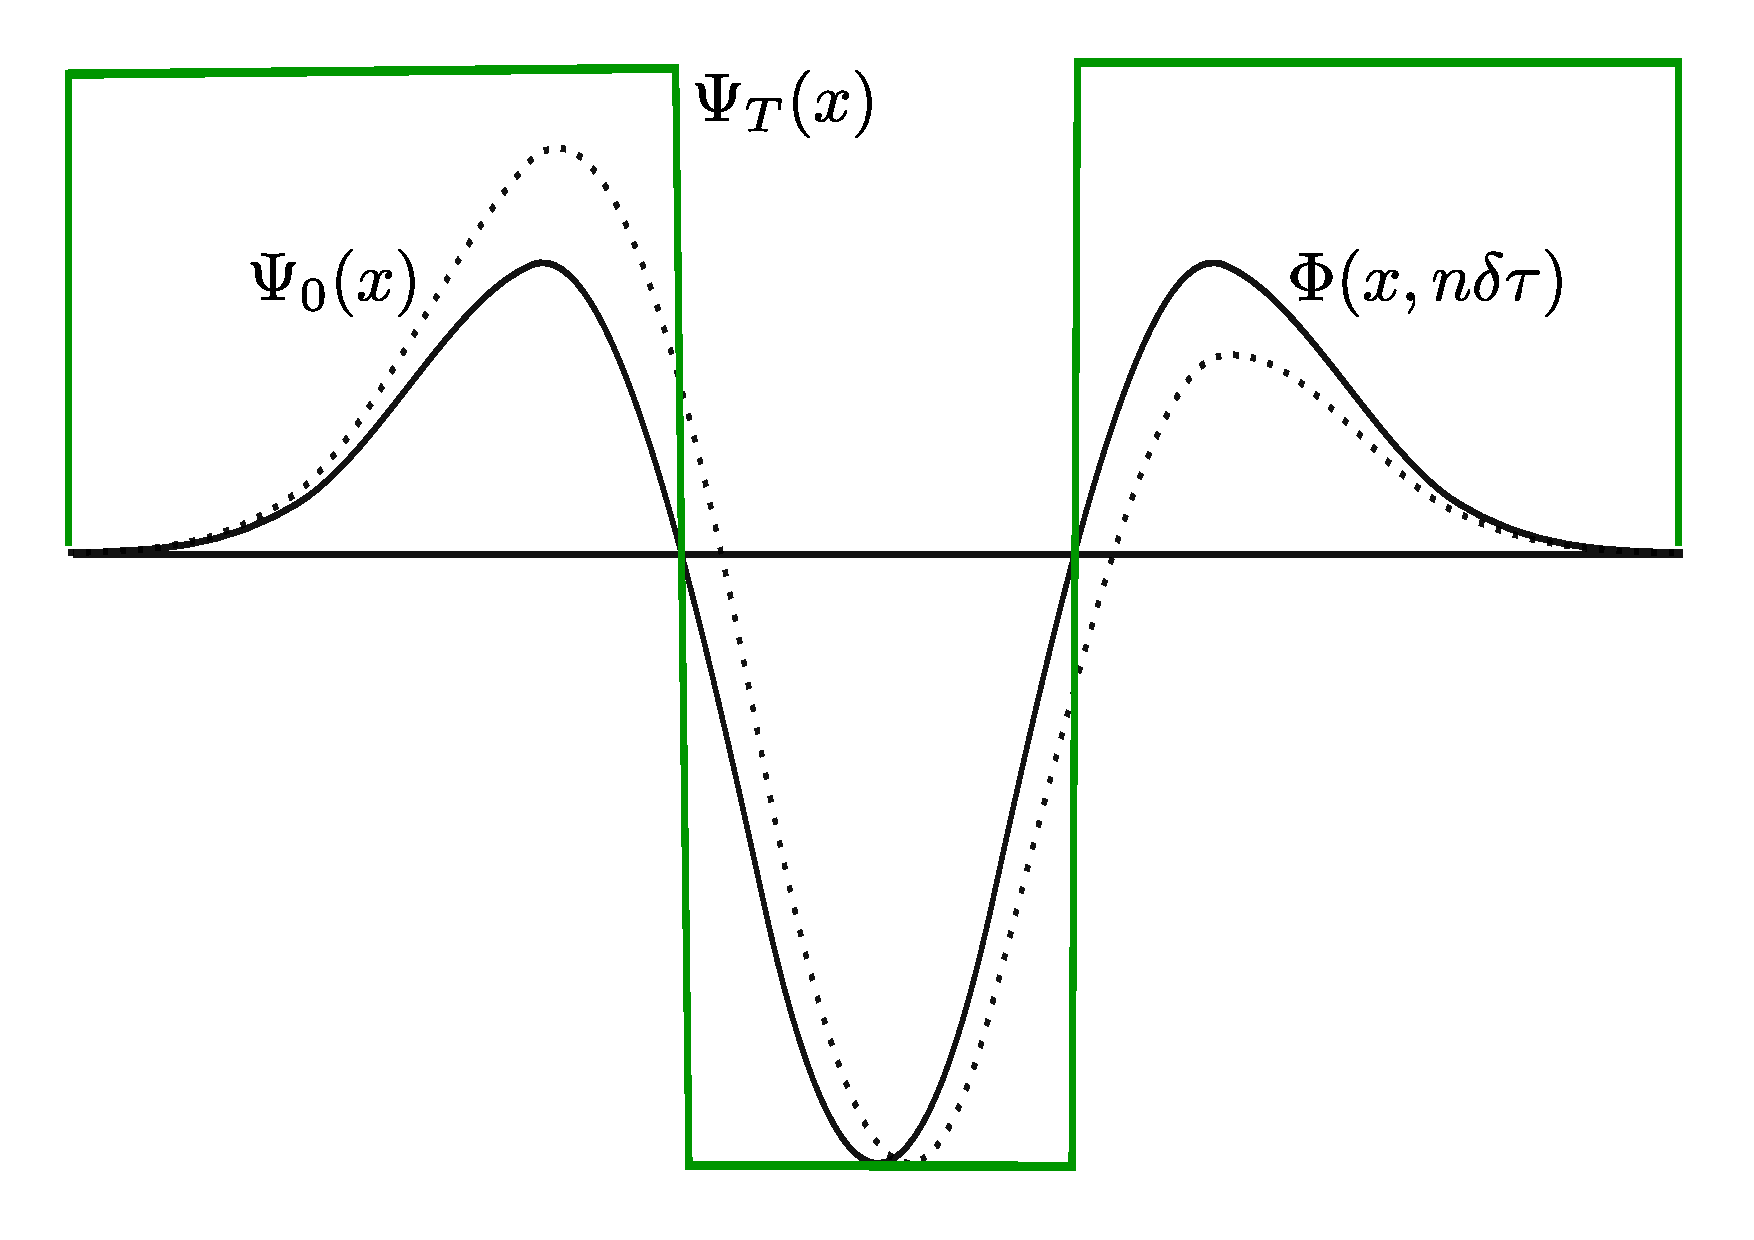
\includegraphics[scale=0.3]{../graphics/fixxednode.pdf}
 \end{center}
 \caption{The fixed node approximation illustrated. The nodes of $\Phi(x, n\delta\tau)$ is fixed to match those of $\Psi_T(x)$.}
\end{figure}
\end{frame}


\begin{frame}
\frametitle{Branching}

\textbf{Idea}: The weights are modelled by spawning and killing walkers with a rate equal to $G_\mathrm{W}$. 
\shift

\textbf{Problem}: $G_\mathrm{W}$ is not necessarily an integer.
\shift

\textbf{Solution}: The walker branch $\mathrm{floor}(G_\mathrm{B})$ times with a chance of one additional copy.


\vspace{0.5cm}
If zero branches, the walker is removed.

% \shift
% 
% Or more compact: Create 
% 
% \begin{equation}
% \overline{G}_\mathrm{B} = \mathrm{floor}(G_\mathrm{B} + a)
% \end{equation}
% 
% copies, where $a \in [0,\,1)$ is a uniformly distributed random number. If the value is zero, the walker dies.

\end{frame}


\begin{frame}
\frametitle{Branching}

\begin{figure}
\begin{center}
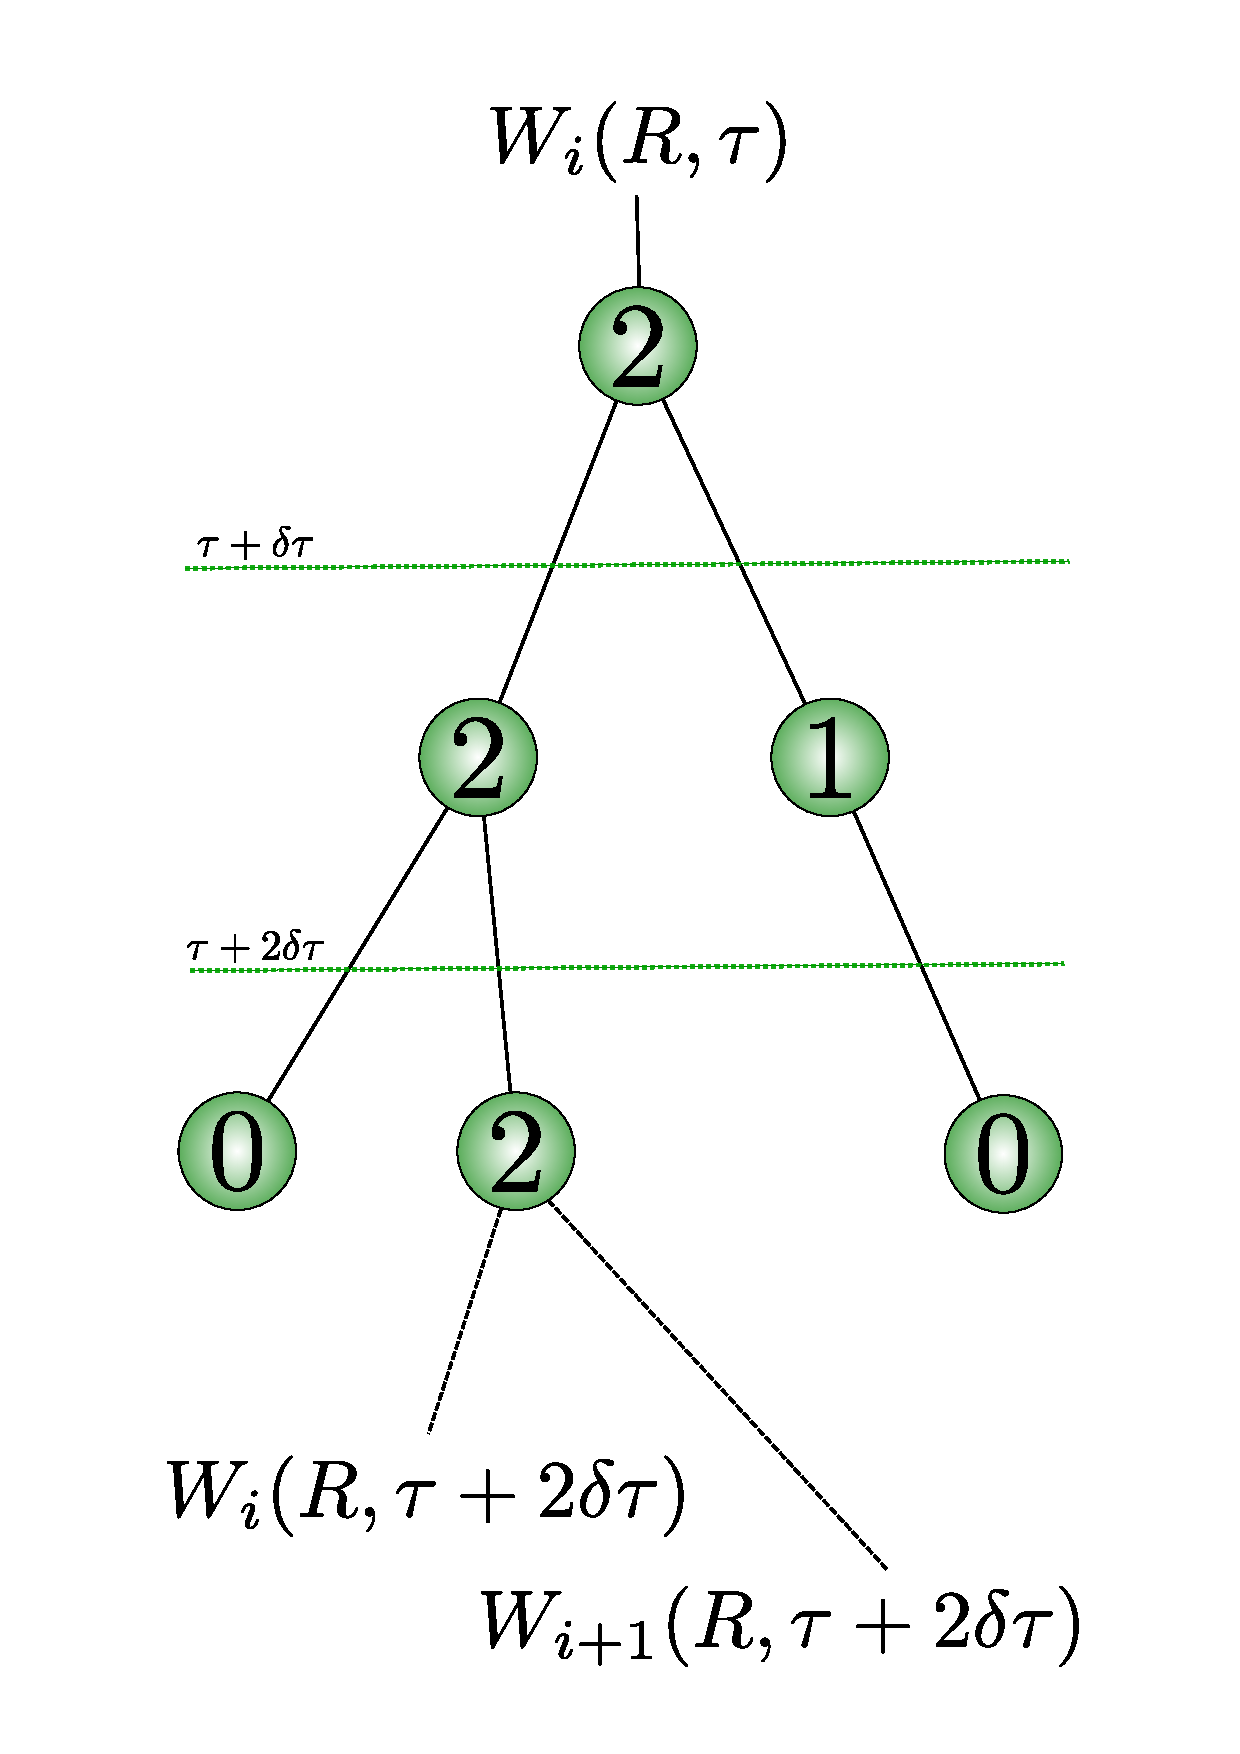
\includegraphics[scale=0.2]{../graphics/branching.pdf}
\end{center}
\caption{Branching illustrated. The integer values represent $\overline{G}_\mathrm{B}$.}
\end{figure}

\end{frame}

\begin{frame}
 \frametitle{Diffusion}
 
%  The diffusion equation representing $G_\mathrm{Diff}$ is the so-called \textit{Fokker-Planck equation}. 
%  \shift
%  
%  Anisotropic diffusion process. The quantum force pushes the walkers into regions of higher probability. 
%  \shift
%  
%  According to the Fokker-Planck formalism, 

According to the introduced diffusion process, the new position $\mathbf{r}_{i+1}$ is calculated from the old one, $\mathbf{r}_i$, as follows
 
 \begin{equation*}
  \mathbf{r}_{i+1} = \mathbf{r}_i + D\delta\tau\mathbf{F}(\mathbf{r}_i) + \mathbf{\xi}, 
 \end{equation*}

where $\mathbf{\xi}$ is a vector of normal distributed random numbers with variance $\sqrt{2D\delta\tau}$.
 
\end{frame}

\begin{frame}
\frametitle{Diffusion}

\textbf{Problem}: Due to a finite time step, the previous equations do not guarantee convergence.  
\shift

\textbf{Solution}: The \textit{Metropolis algorithm} will correct this bias:  

\begin{equation*}
  A(i\,\rightarrow\,j) = \min\{R_G(i\,\rightarrow\,j)R_\psi(i\,\rightarrow\,j)^2, \,1\},
\end{equation*}

where $i\,\rightarrow\,j$ denotes a transition from state $i$ to state $j$, $A$ is the probability of accepting the transition, 

\begin{equation*}
 R_G(i\,\rightarrow\,j) = G_\mathrm{Diff}(\mathbf{r}_{j}, \mathbf{r}_{i}; \delta\tau)/G_\mathrm{Diff}(\mathbf{r}_{i}, \mathbf{r}_{j}; \delta\tau),
\end{equation*}

and

\begin{equation*}
 R_\psi(i\,\rightarrow\,j) = |\Psi_T(\mathbf{r}_j)/\Psi_T(\mathbf{r}_i)|.
\end{equation*}

\end{frame}


%% 15

\begin{frame}
 \frametitle{Recap}
 
 \begin{itemize}
 \item The distribution at any stage is given as the histogram of the walkers' configurations.
 \pause \item The projection process involves diffusing the walkers and calculating weights.
 \pause \item Efficient sampling by using the quantum force.
 \pause \item Unbiased sampling by using the Metropolis algorithm.
 \pause \item Transition from $|\Psi_T|^2 \to f(\mathbf{r}, \tau)$ by including the weights.
%  \pause \item The Metropolis algorithm corrects the bias introduced by a finite step length. Ensures that the walkers follow $|\Psi_T(\mathbf{r})|^2$.
%  \pause \item After each diffusion step, the walker is either killed or cloned based on the value of the branching Green's function. This ensures that the distribution of walkers follows $f(\mathbf{r}, \tau)$ and not $|\Psi_T(\mathbf{r})|^2$.
 \end{itemize}

\end{frame}

\subsection{Explicit methods}

\begin{frame}
 \frametitle{Variational Monte-Carlo}
 Neglecting the branching results in a method known as \textit{Variational Monte-Carlo} (VMC).
 \shift
 
 Corresponds to calculating $\bra{\Psi_T}\OP{H}\ket{\Psi_T}$ using a standard Monte-Carlo approach
 
 \begin{equation*}
  \bra{\Psi_T}\OP{H}\ket{\Psi_T} = \int_\mathbf{r} |\Psi_T(\mathbf{r})|^2 E_L(\mathbf{r})\mathrm{d}\mathbf{r} \simeq \frac{1}{N}\sum_{i=1}^N \frac{1}{\Psi_T(\mathbf{r_i})}\OP{H}\Psi_T(\mathbf{r}_i) 
 \end{equation*}
 
\end{frame}

\begin{frame}
 \frametitle{\textbf{Variational} Monte-Carlo}
 
 Variational Monte-Carlo will always result in an energy which is greater or equal to the exact ground state energy
 
 \begin{align*}
  \bra{\Psi_T}\OP{H}\ket{\Psi_T} &= \sum_{ij} C_i^\ast C_j \underbrace{\bra{\Psi_i} \OP{H} \ket{\Psi_j}}_{E_i\delta_{ij}} \\
                                 &= \sum_i |C_i|^2 E_i \\
                                 &= \sum_i |C_i|^2 (E_0 + \Delta E_i) \\
                                 &= E_0 \underbrace{\sum_i |C_i|^2}_{1} + \underbrace{\sum_i |C_i|^2\Delta E_i}_{\ge 0} \\
                                 &\ge E_0.
 \end{align*}
\end{frame}

\begin{frame}
 \frametitle{Limitations: VMC}
 
 VMC is extremely robust, however, extremely dependent on a good ansatz for $\Psi_T(\mathbf{r})$.
 
\end{frame}



\begin{frame}
 \frametitle{Limitations: VMC}
 
 \begin{figure}
  \begin{center}
   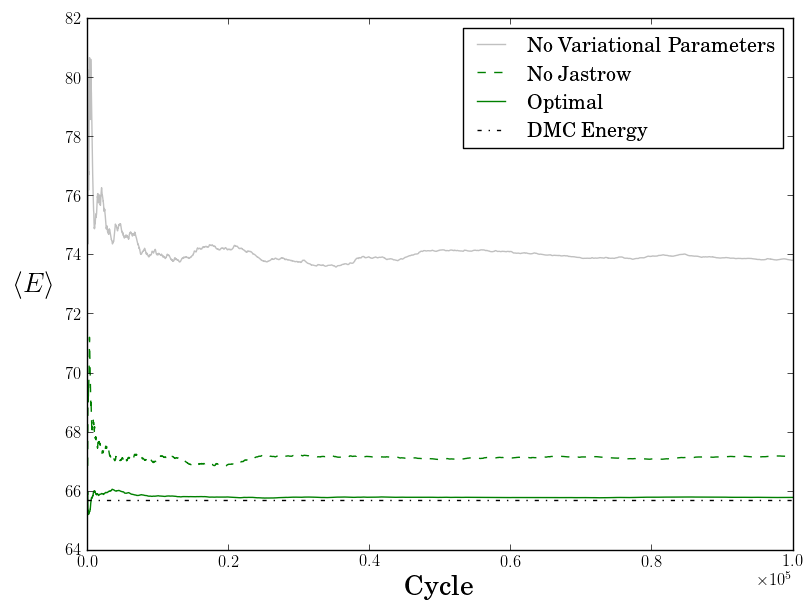
\includegraphics[scale=0.35]{../graphics/WFComp.png}
  \end{center}
  \caption{Comparison of different trial wave functions for a two-dimensional 12-particle quantum dot with unit frequency.}
 \end{figure}
 
\end{frame}

% \begin{frame}
%  The \textit{variational principle} introduced in the previous slide opens up the possibility to introduce \textit{variational parameters} in $\Psi_T(\mathbf{r})$ whose values are found by minimizing the VMC energy in the parameter space.
%  \shift
%  
%  Already have $\beta$ from the Jastrow factor. 
%  \shift
%  
%  The \textit{spatial} wave function is modelled as a single \textit{Slater determinant}, which can be split into two parts $|\mathbf{S(\mathbf{r})}^\uparrow|$ and $|\mathbf{S(\mathbf{r})}^\downarrow|$ corresponding to two spin levels due to the fact that the Hamiltonian is assumed to be \emph{spin independent}.
%  \shift
%  
%  Introducing the variational parameter $\alpha$ into the spatial wave function yields
%  
%  
%  \begin{equation}
%   \Psi_T(\mathbf{r}; \alpha, \beta) = |\mathbf{S(\mathbf{r}; \alpha)}^\uparrow||\mathbf{S(\mathbf{r}; \alpha)}^\downarrow|J(\mathbf{r}; \beta)
%  \end{equation}
% 
%  
%  
% \end{frame}

\begin{frame}
\frametitle{Diffusion Monte-Carlo}
Including both diffusion and branching results in a method known as \textit{Diffusion Monte-Carlo} (DMC).
\shift

The DMC energy corresponds to the following integral

\begin{equation*}
 E_{\mathrm{DMC}} = \frac{\int_\mathbf{r} f(\mathbf{r}, \tau) \frac{1}{\Psi_T(\mathbf{r})}\OP{H} \Psi_T(\mathbf{r})\mathrm{d}\mathbf{r}}{\int_\mathbf{r} f(\mathbf{r}, \tau)\mathrm{d}\mathbf{r}}  = \frac{\bra{\Phi(\tau)} \OP{H} \ket{\Psi_T}}{\braket{\Phi(\tau)}{\Psi_T}},
\end{equation*}

\pause
which upon convergence of the projection results in $\OP{H}\ket{\Phi(\tau)} = E_0\ket{\Phi(\tau)}$. The energy becomes

\begin{equation*}
 E_{\mathrm{DMC}} = \frac{\bra{\Phi(\tau)}E_0\ket{\Psi_T}}{\braket{\Phi(\tau)}{\Psi_T}} = E_0.
\end{equation*}

\end{frame}




\begin{frame}
  \frametitle{Limitations: DMC}
  
  As discussed previously: The fixed node approximation.
  \shift
  
  The branching can get out of control for high \textit{variance} systems. 
  \shift
  
  Can be countered by choosing a lower time step. 
  
  \begin{equation*}
   G_W \sim \exp(\sigma(E)\delta\tau)
  \end{equation*}
  \shift
  
  Low $\delta\tau$ means slower convergence. Unable to span the whole space.
  
\end{frame}

\begin{frame}
   \frametitle{Limitations: DMC}
   
   Diffusion Monte-Carlo is not as dependent on the trial wave function as VMC.
   
\end{frame}

\begin{frame}
 \begin{figure}
  \begin{center}
   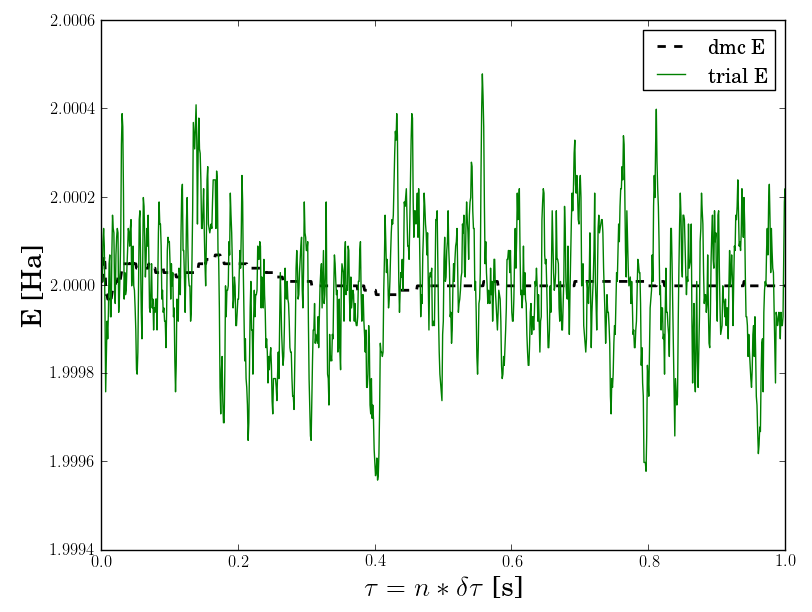
\includegraphics[scale=0.35]{../graphics/DMC_notExactWF.png}
  \end{center}
  \caption{DMC calculation without the exact wave function. The exact result is $E_0=2$. The VMC energy is $2.0042(3)$, whereas the DMC energy is $2.00000(2)$.}
 \end{figure}
\end{frame}








% \section{Live Demo}

\subsection{HallaLive}

\begin{frame}
 Beskriv og vis minimering av trial wave function real time.
 Beskriv og vis VMC + blockingprosessen real-time.
 Vis VMC qdots 2d vmc og DMC real time konvergens.
 vis skalering
 showoff distribusjoner?
\end{frame}
\section{Modelled systems}

\begin{frame}
 \frametitle{The modelled systems}
 \begin{itemize}
  \item Quantum dots: Confined electrons
  \begin{itemize}
  \item Two dimensions
  \item Three dimensions
  \item Double wells
  \end{itemize}
  \pause
  \item Atomic systems
  \begin{itemize}
  \item Atoms
  \item Homonuclear Diatomic Molecules
  \end{itemize}
 \end{itemize}
\end{frame}

\subsection{Quantum dots}

\begin{frame}
 \frametitle{Quantum dots}
 
 Model the confinement using a harmonic oscillator potential
 
 \begin{equation*}
  V_\mathrm{ext}(\mathbf{r}) = \frac{1}{2}\omega^2r^2,
 \end{equation*}
 
 where $\omega$ is the oscillator frequency.
 
 \pause
 
 The harmonic oscillator eigenfunctions are
 
 \begin{equation*}
  \phi_{n_x, n_y, n_z}(\mathbf{r}) = H_{n_x}(\sqrt{\omega}x)H_{n_y}(\sqrt{\omega}y)H_{n_z}(\sqrt{\omega}z)e^{-\frac{1}{2}\omega r^2},
 \end{equation*}
 
 which serves as the starting ground for creating an ansatz for $\Psi_T(\mathbf{r})$.


 
\end{frame}

% \begin{frame}
%  \frametitle{Quantum dots}
%  
%  Introducing a variational parameter $\alpha$ yields
%  
%  \begin{equation}
%   \phi_{n_x, n_y, n_z}(\mathbf{r}; \alpha) = H_{n_x}(kx)H_{n_y}(ky)H_{n_z}(kz)e^{-\frac{1}{2}k^2r^2},
%  \end{equation}
%  
%  where $k = \sqrt{\alpha\omega}$ represents the scaled oscillator potential.
%  \shift
% 
%  \textbf{Problem}: With the electron-electron interaction these are no longer eigenfunctions of the Hamiltonian.
%  \shift
%  
%  \textbf{Solution}: Quantum Monte-Carlo!
%  
% \end{frame}

\begin{frame}
 \begin{figure}
 \begin{center}
  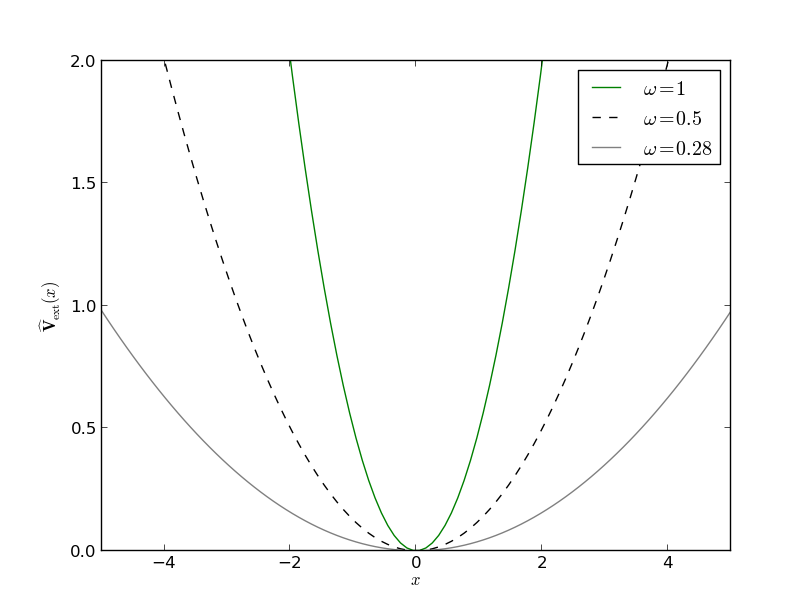
\includegraphics[scale=0.4]{../graphics/Potentials/qdots.png}
  \caption{A one-dimensional version of the single-particle potential of quantum dots.}
  \label{fig:extPotQDOTS}
 \end{center}
\end{figure}
\end{frame}

% \begin{frame}
%  \frametitle{Double wells}
%  
%  The double-well potential used is
%  
%  \begin{equation}
%   V_\mathrm{ext}(\mathbf{r}) = \frac{1}{2}m^\ast \omega_0^2 \left[r^2 + \frac{1}{4}R^2 - R|x|\right], 
%  \end{equation}
% 
%  where $R$ is the well separation, and $m^\ast$ and $\omega_0$ are material constants.
%  \shift
%  
%  The construction of the new basis will be discussed later.
%  
% \end{frame}

\begin{frame}
\frametitle{Double wells}
 \begin{figure}
 \begin{center}
  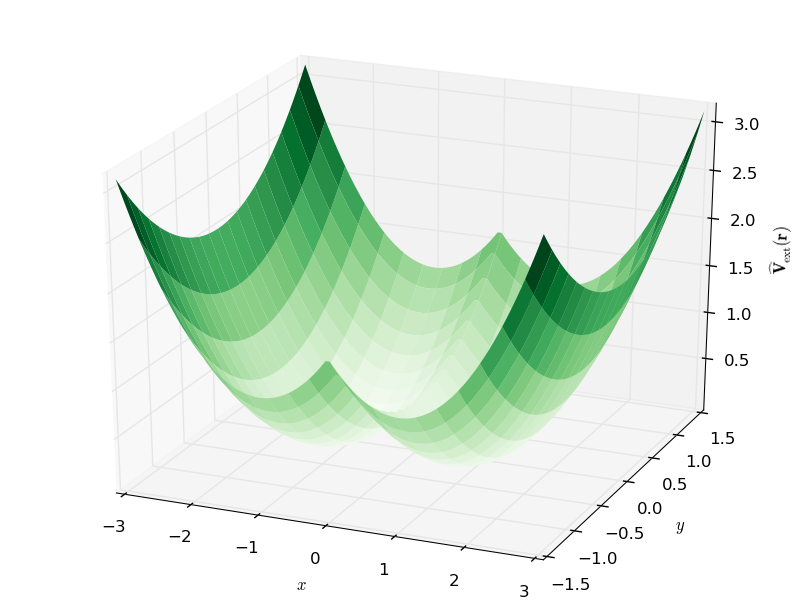
\includegraphics[scale=0.4]{../graphics/Potentials/doubleWell.png}
  \caption{The external potential for a double-well quantum dot.}
  \label{fig:extPotDoubleWell}
 \end{center}
\end{figure}
\end{frame}

\subsection{Atomic systems}

\begin{frame}
 \frametitle{Atomic systems}
 
Atoms are modelled with a Coulomb interaction between the electrons and the nucleus 
 
 \begin{equation*}
 V_\mathrm{ext}(\mathbf{r}) = -\frac{Z}{r}. \label{eq:v0hydro}
\end{equation*}
\vspace{0.5cm}
 
The nucleus is fixed at the origin (the \textit{Born-Oppenheimer Approximation}).
 
\end{frame}

\begin{frame}
\begin{figure}
 \begin{center}
  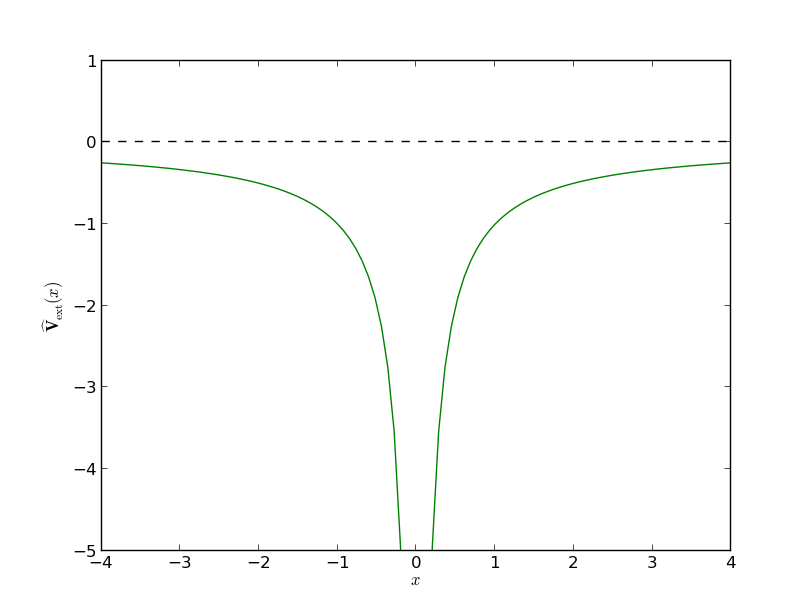
\includegraphics[scale=0.4]{../graphics/Potentials/hydrogen.png}
  \caption{The one-dimensional version of the single-particle potential of hydrogen.}
  \label{fig:extPotHydrogen}
 \end{center}
\end{figure}
\end{frame}

\begin{frame}
 The eigenfunctions are
 
 \begin{equation*}
 \phi_{nlm}(r, \theta, \phi; Z) \propto r^l e^{-Zr/n}\left[L_{n-l-1}^{2l+1}\left(\frac{2r}{n}Z\right)\right] Y_l^m(\theta, \phi).
\end{equation*}

$L_{q-p}^p(x)$: \textit{Associated Laguerre polynomials} \\
$Y_l^m(\theta, \phi)$: \textit{Spherical harmonics}. 
% \shift
% The spherical harmonics are related to the \textit{associated Legendre functions} $P_l^m$ in the following manner:
% 
% \begin{equation}
%  Y_l^m(\theta, \phi) \propto   P_l^m(\cos\theta)e^{im\phi}. \label{eq:spherHarm}
% \end{equation}

\end{frame}

\begin{frame}
 \textbf{Issue}: The spherical harmonics are complex functions. 
 \shift
 \textbf{Solution}: Use the \textit{solid harmonics}
 
 \begin{align*}
S_l^m(r, \theta, \phi) &\propto r^l\left[Y_l^m(\theta, \phi) + (-1)^m Y_l^{-m}(\theta, \phi)\right] \\
 &\propto r^{l} P_l^{|m|}(\cos\theta) \begin{cases} \cos m\phi & m \ge 0 \\ \sin|m|\phi &  m < 0 \end{cases}.     
\end{align*}

 \end{frame}
 
 \begin{frame}
  The resulting eigenfunctions become 
  
\begin{equation*}
  \phi_{nlm}(r, \theta, \phi; Z) \propto e^{-Zr/n}\left[L_{n-l-1}^{2l+1}\left(\frac{2r}{n}Z\right)\right] S_l^m(r, \theta, \phi) \equiv \phi^\mathrm{H}_{nlm}(\mathbf{r}).
\end{equation*}
 \end{frame}

 \begin{frame}
 \frametitle{Molecules}
 \begin{figure}
 \begin{center}
  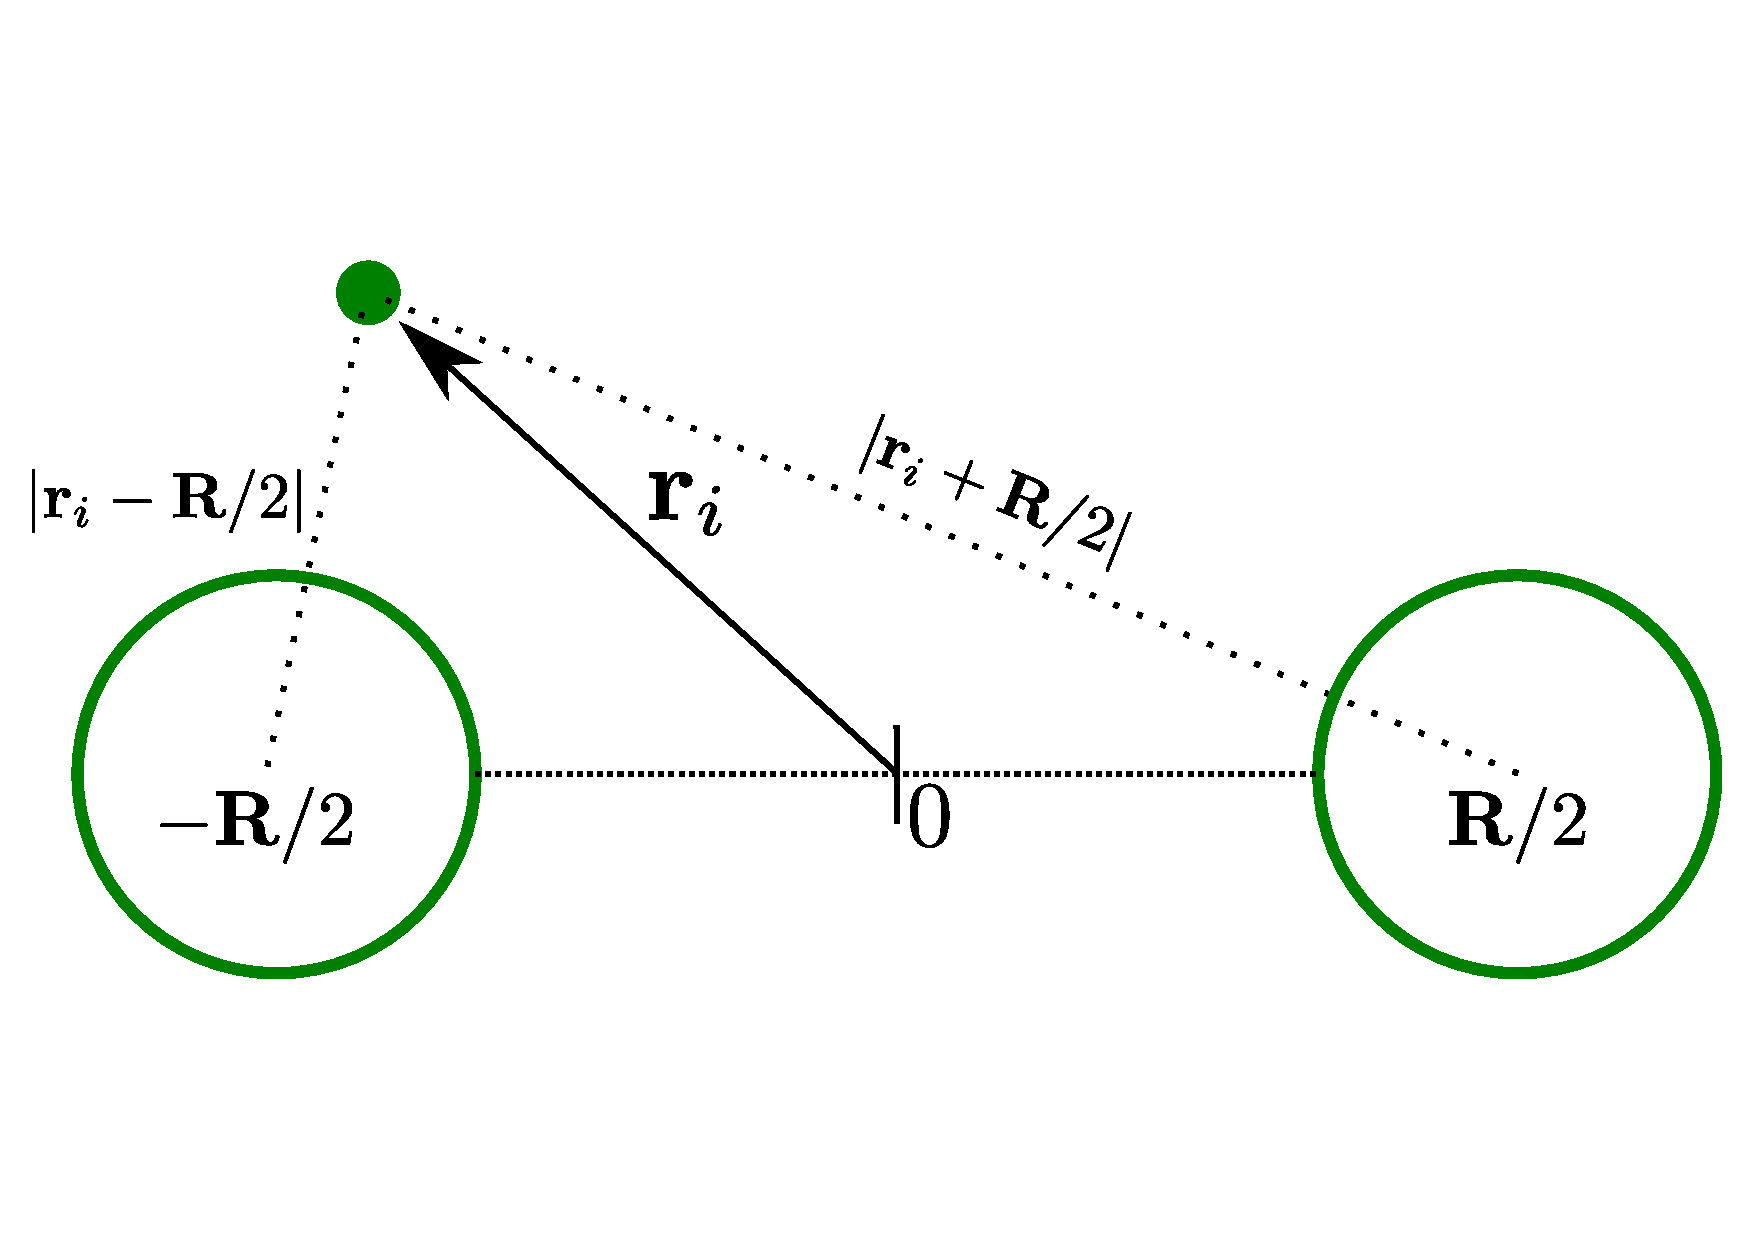
\includegraphics[scale=0.3]{../graphics/Molecules.pdf}
  \caption{The model for the diatomic molecule.}
 \end{center}
\end{figure}
\end{frame}
 
\begin{frame}
 
 The Hamiltonian describing the homonuclear diatomic molecules becomes
 
 \begin{equation*}
 \OP{H}_{\mathrm{Mol.}}(\mathbf{r}, \mathbf{R}) = \sum_{i=1}^N \left[-\frac{1}{2}\nabla_i^2 + \frac{Z}{|\mathbf{r}_i + \mathbf{R}/2|} + \frac{Z}{|\mathbf{r}_i - \mathbf{R}/2|}\right] + \frac{Z^2}{R} + \sum_{i<j} \frac{1}{r_{ij}}.
\end{equation*}
 
\end{frame}



\begin{frame}
%  In order to transform the hydrogen eigenstates $\phi_{nlm}^\mathrm{H}(\mathbf{r})$, which are symmetric around a single nucleus, into molecular single-particle states $\phi_{nlm}^\pm (\mathbf{r}_i)$, a superposition of the two mono-nucleus wave functions are used:

 A transformation of the single-nucleus hydrogen eigenstates are needed:
 
\begin{align*}
 \phi_{nlm}^+ (\mathbf{r}_i, \mathbf{R}) &= \phi_{nlm}^\mathrm{H}(\mathbf{r}_i + \mathbf{R}/2) + \phi_{nlm}^\mathrm{H}(\mathbf{r}_i - \mathbf{R}/2)\label{eq:moleculeTransPlus}, \\
 \phi_{nlm}^- (\mathbf{r}_i, \mathbf{R}) &= \phi_{nlm}^\mathrm{H}(\mathbf{r}_i + \mathbf{R}/2) - \phi_{nlm}^\mathrm{H}(\mathbf{r}_i - \mathbf{R}/2)\label{eq:moleculeTransMin}.
\end{align*}
\shift 

The same transformation is used to transform the harmonic oscillator eigenfunctions into the double well basis.

\end{frame}




\section{Results and Discussions}

\subsection{Quantum Dots}

\begin{frame}


%Two particle 2D
\begin{figure}
 \begin{center}
 \begin{tabular}{c|lll}
  $\omega$ & $\mathrm{E_{VMC}}$ & $\mathrm{E_{DMC}}$ & $\mathrm{E_{FCI}}$\\
\hline\hline
\multicolumn{4}{c}{} \\
 0.01   & \textbf{0.07}406(5)  & \textbf{0.07383}9(2)  & 0.07383505 \\
 0.1    & \textbf{0.44}130(5)  & \textbf{0.44079}(1)   & 0.44079191 \\
 0.28   & \textbf{1.02}215(5)  & \textbf{1.02164}(1)   & 1.0216441  \\
 0.5    & \textbf{1.6}6021(5)  & \textbf{1.65977}(1)   & 1.6597723  \\
 1.0    & \textbf{3.000}30(5)  & \textbf{3.00000}(1)   & 3.0000001  \\
\cline{1-4}
 \end{tabular}  
 \end{center}
  \caption{Two-particle results for two-dimensional quantum dots compared with FCI results by Veronica K.B. Olsen.}
\end{figure}
\end{frame}


%Two particle 42 56 2D
\begin{frame}

\begin{figure}
 \begin{center}
 \footnotesize
 \begin{tabular}{cc|llll}
 N      &  $\omega$ & $\mathrm{E_{VMC}}$ & $\mathrm{E_{DMC}}$ & $\mathrm{E_{SRG}}$ & $\mathrm{E_{CCSD}}$\\
\hline\hline
\multicolumn{6}{c}{} \\
    42    &   0.1    & 107.881(1)  & 107.6389(2) &- 			& 111.7170  \\
          &   0.28   & 220.161(1)  & 219.8426(2) &219.8836 	& 222.1401  \\
          &   0.5    & 331.002(1)  & 330.6306(2) &330.6485	& 331.8901  \\
          &   1.0    & 544.2(8)    & 542.9428(8) &542.9528 	& 543.1155 \\
\cline{2-6}
\multicolumn{6}{c}{} \\
    56    &   0.1    & 176.269(2) & 175.9553(7)  & -		& 186.1034 \\
          &   0.28   & 358.594(2) & 358.145(2)   & -		& 363.2048  \\
          &   0.5    & 538.5(6)   & 537.353(2)   & -		& 540.3430 \\
          &   1      & 880.2(7)   & 879.3986(6)  & -		& 879.6386 \\
\cline{2-6}
 \end{tabular}  
 \end{center}
  \caption{Results for two-dimensional quantum dots 42 and 56 particles compared with SRG results by Sarah Reimann and CCSD results by Christoffer Hirth.}
\end{figure}
\end{frame}

\normalsize

%Two particle 2D
\begin{frame}

\footnotesize
\begin{figure}
 \begin{center}
 \begin{tabular}{cc|rrr}
    N     & $\omega$ & $\mathrm{E_{VMC}}$ & $\mathrm{E_{DMC}}$ & $\mathrm{E_0}$\\
\hline\hline
\multicolumn{5}{c}{} \\
    2     &   0.01   & 0.07939(3)  & 0.079206(3) & -		\\
          &   0.1    & 0.50024(8)  & 0.499997(3) & 0.5        \\
          &   0.28   & 1.20173(5)  & 1.201725(2) & -		\\
          &   0.5    & 2.00005(2)  & 2.000000(2) & 2.0 \\
          &   1.0    & 3.73032(8)  & 3.730123(3) & - \\
% \cline{2-5}
% \multicolumn{5}{c}{} \\
%     8     &   0.1    & 5.7130(6)   & 5.7028(1)   & - 		\\
%           &   0.28   & 12.2040(8)  & 12.1927(1)  & -		\\
%           &   0.5    & 18.9750(7)  & 18.9611(1)  & -\\
%           &   1.0    & 32.6842(8)  & 32.6680(1)  & -\\
% \cline{2-5}
% \multicolumn{5}{c}{} \\
%     20    &   0.1    & 27.316(2)   & 27.2717(2)   & - 		\\
%           &   0.28   & 56.440(2)   & 56.3868(2)   & -		\\
%           &   0.5    & 85.714(2)   & 85.6555(2)   & - \\
%           &   1.0    & 142.951(2)  & 142.8875(2)  & -
 \end{tabular}  
 \end{center}
  \caption{Results for three-dimensional quantum dots compared with exact solutions by M. Taut.}
\end{figure}
\end{frame}

\normalsize


 
 \begin{frame}
  \captionsetup[subfloat]{labelformat=empty}
\begin{figure}
 \begin{center}
  \subfigure[$N=2$]{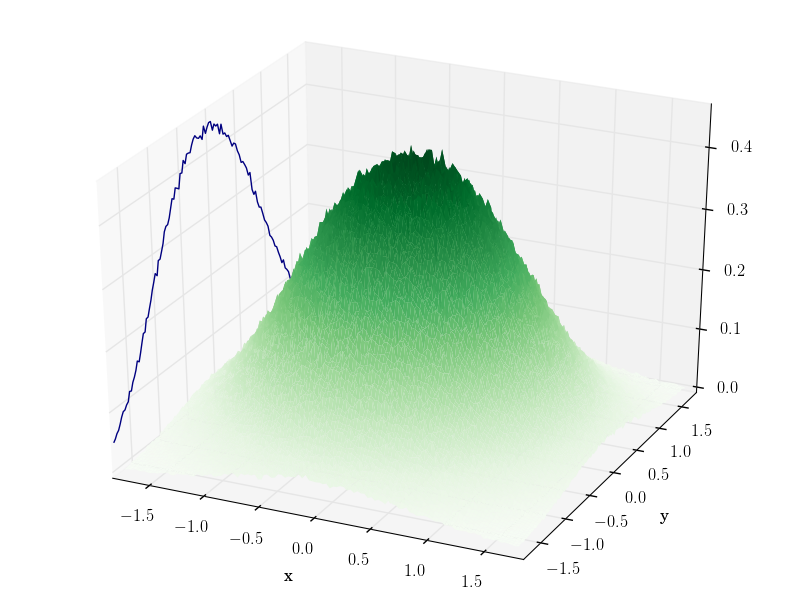
\includegraphics[scale=0.15]{../graphics/OBD/OBD_DMC/dist_out_QDots2c1_3D.png}}
  \subfigure[$N=12$]{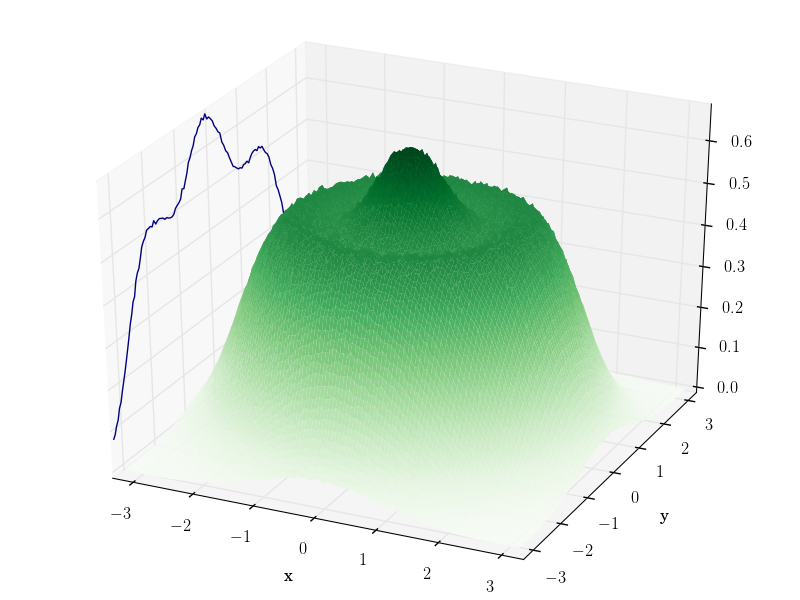
\includegraphics[scale=0.15]{../graphics/OBD/OBD_DMC/dist_out_QDots12c1_3D.png}}
  \subfigure[$N=30$]{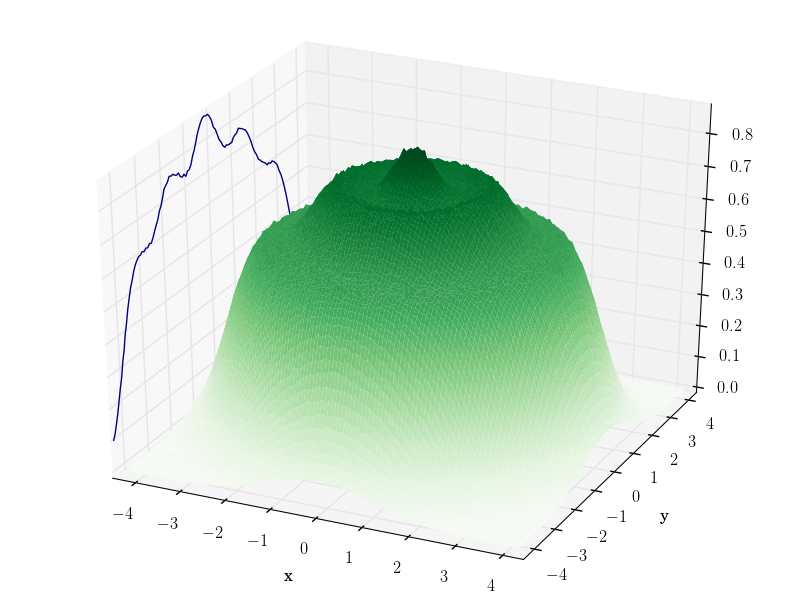
\includegraphics[scale=0.15]{../graphics/OBD/OBD_DMC/dist_out_QDots30c1_3D.png}}\\
  \subfigure[$N=6$]{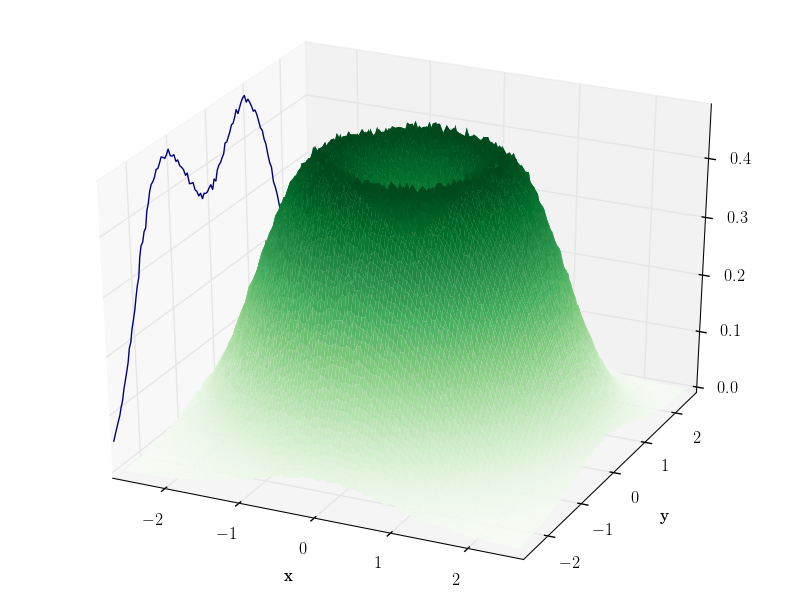
\includegraphics[scale=0.15]{../graphics/OBD/OBD_DMC/dist_out_QDots6c1_3D.png}} 
  \subfigure[$N=20$]{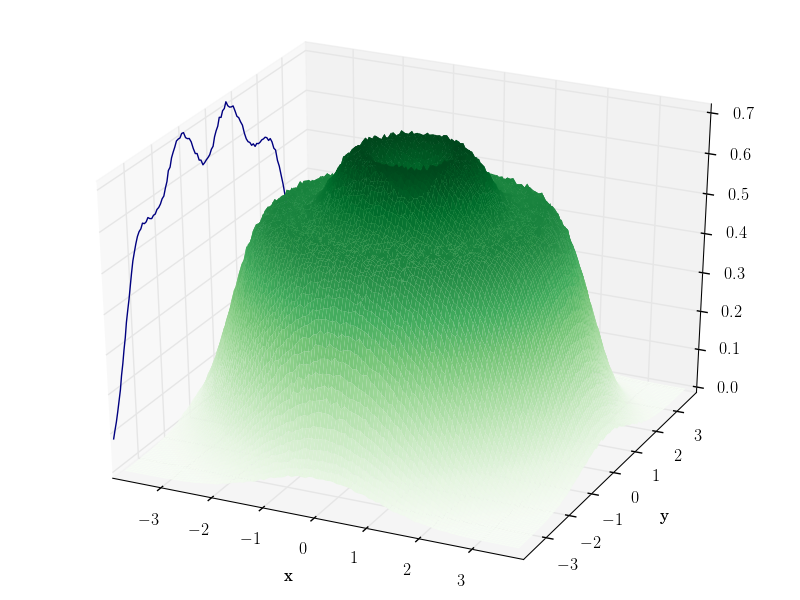
\includegraphics[scale=0.15]{../graphics/OBD/OBD_DMC/dist_out_QDots20c1_3D.png}} 
  \subfigure[$N=42$]{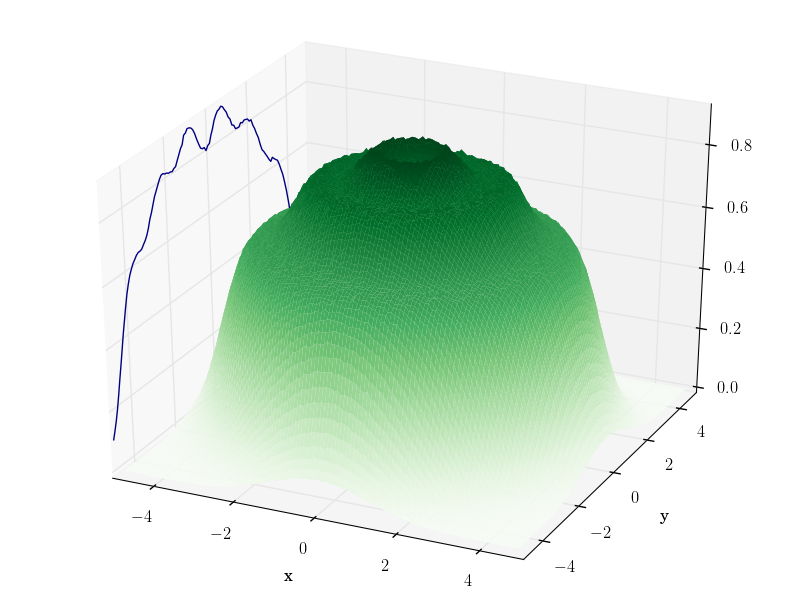
\includegraphics[scale=0.15]{../graphics/OBD/OBD_DMC/dist_out_QDots42c1_3D.png}} \\
  \caption{DMC one-body densities for two-dimensional quantum dots.}
  \label{fig:OBD_DMC_QDOTS_w1} 
 \end{center}
\end{figure}
 \end{frame}

% \begin{frame}

% \begin{center}
% \begin{tabular}{cc}
% VMC density & $|\Psi_T(\mathbf{r})|^2$ \\
% &  \\
% DMC density & $\Phi(\mathbf{r}, \tau)\Psi_T(\mathbf{r})$ \\
% &  \\
% Pure density & $|\Phi(\mathbf{r}, \tau)|^2$  
% \end{tabular}
% \end{center}

% \end{frame}
 
\begin{frame}

\begin{figure}
 \begin{center}
 \begin{tabular}{cc|c}
   \subfigure{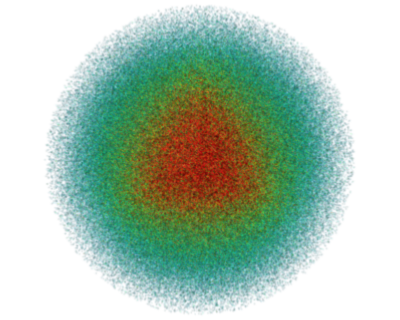
\includegraphics[scale=0.15]{../graphics/OBD/OBD_Q3D/QD2w1_3D.png}} &
   \subfigure{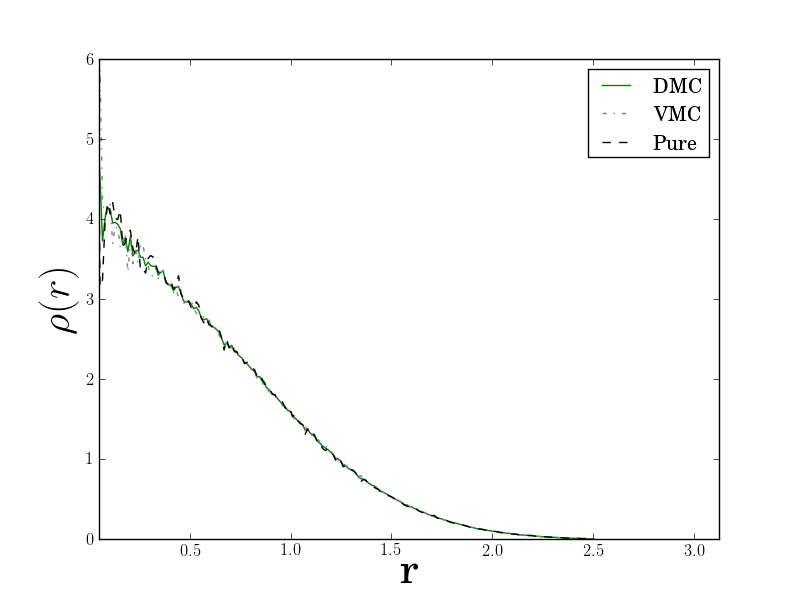
\includegraphics[scale=0.12]{../graphics/OBD/OBD_Q3D/QD2w1_2D.png}} &
   \subfigure{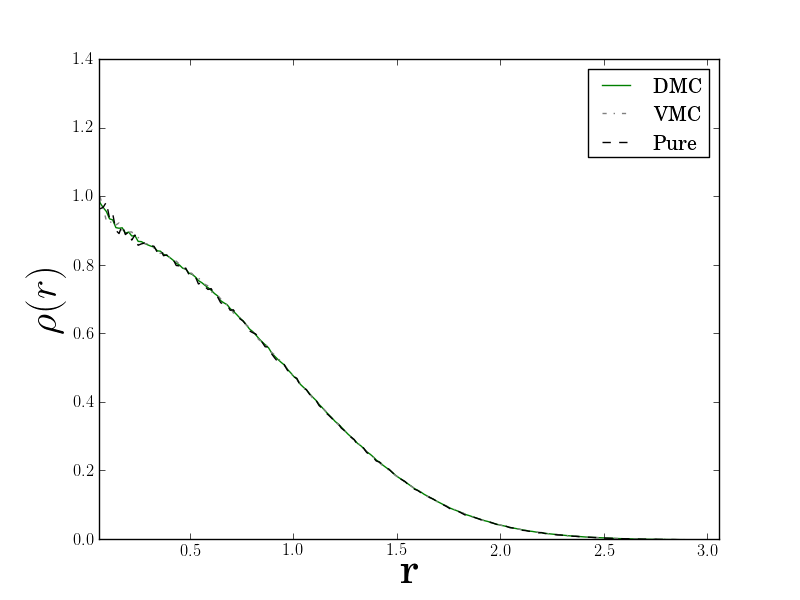
\includegraphics[scale=0.12]{../graphics/OBD/OBD_Q3D/comp/Q2D_2.png}} \\
   \subfigure{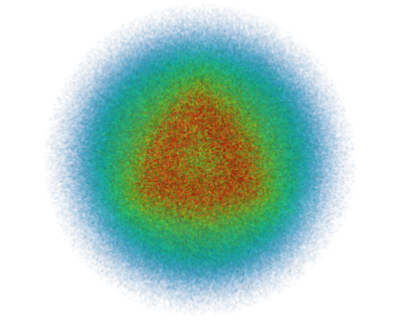
\includegraphics[scale=0.15]{../graphics/OBD/OBD_Q3D/QD8w1_3D.png}} &
   \subfigure{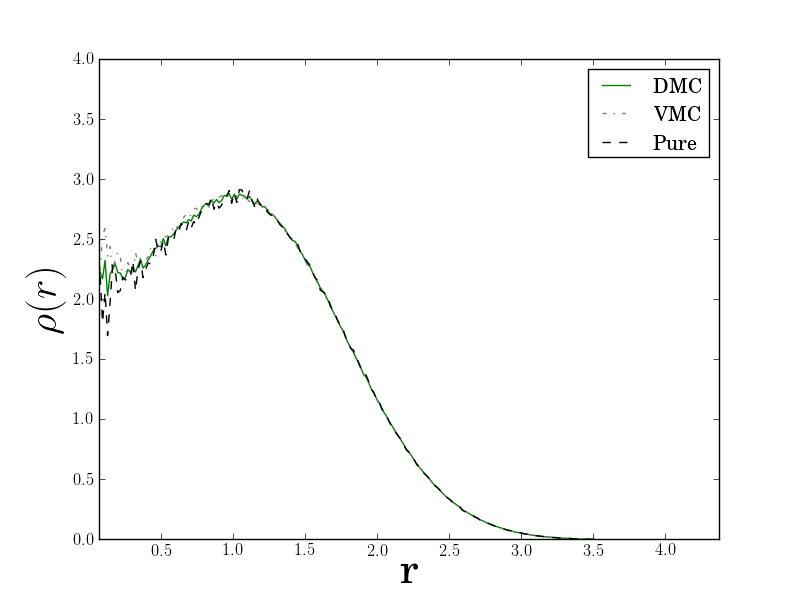
\includegraphics[scale=0.12]{../graphics/OBD/OBD_Q3D/QD8w1_2D.png}} & 
   \subfigure{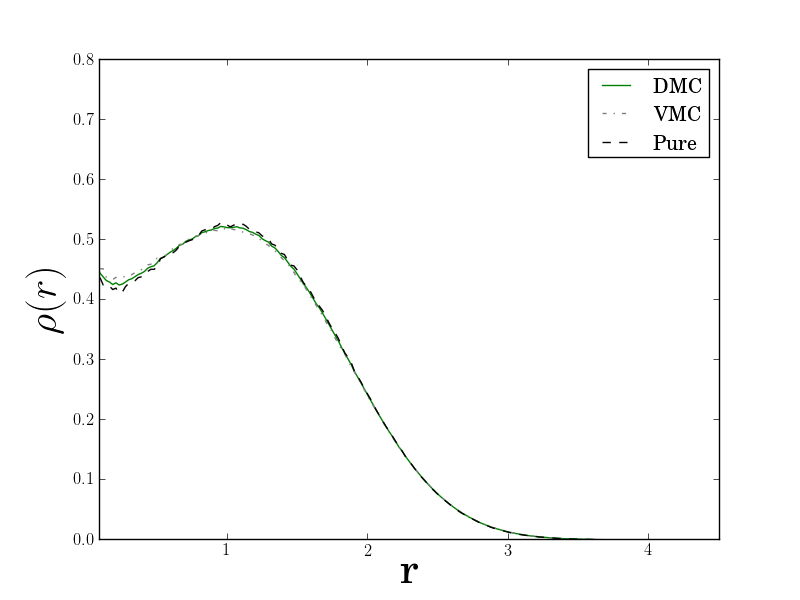
\includegraphics[scale=0.12]{../graphics/OBD/OBD_Q3D/comp/Q2D_6.png}} \\
   \subfigure{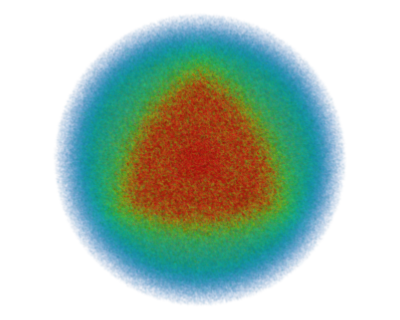
\includegraphics[scale=0.15]{../graphics/OBD/OBD_Q3D/QD20w1_3D.png}} &
   \subfigure{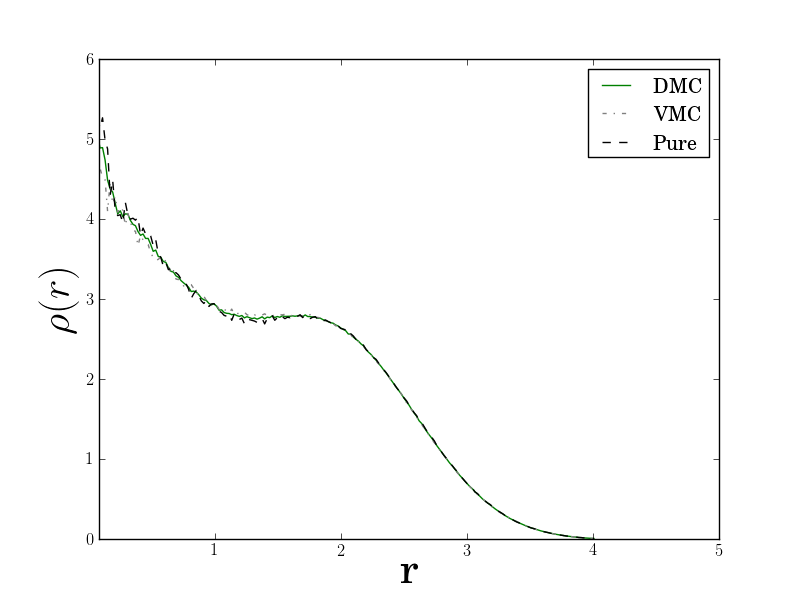
\includegraphics[scale=0.12]{../graphics/OBD/OBD_Q3D/QD20w1_2D.png}} & 
   \subfigure{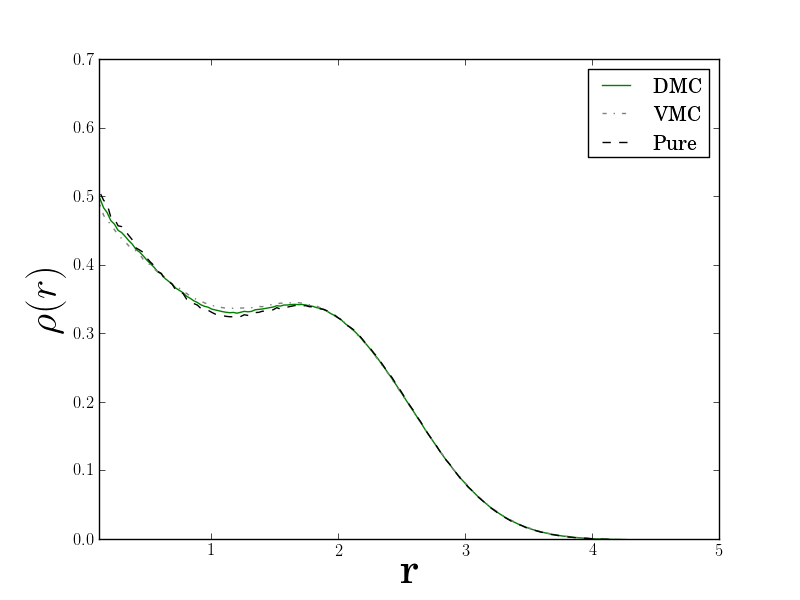
\includegraphics[scale=0.12]{../graphics/OBD/OBD_Q3D/comp/Q2D_12.png}} \\
  \end{tabular}
  \caption{One-body densities for two- and three-dimensional quantum dots.}
  \label{fig:OBD_QDOTS3D_highfreq}
 \end{center}
\end{figure}

\end{frame}


\begin{frame}
\frametitle{Lowering the frequency}

\setlength{\tabcolsep}{0.1pt}
\def\arraystretch{0}
\begin{figure}
 \begin{center}
 \begin{tabular}{rl}
   \footnotesize{\rot{$\qquad\omega=1$}}&\subfigure{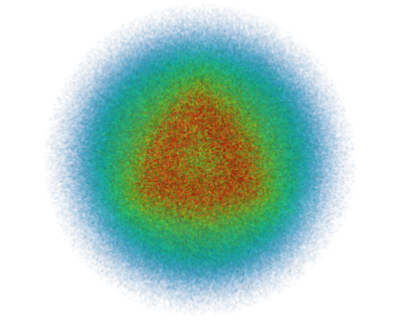
\includegraphics[scale=0.2]{../graphics/OBD/OBD_Q3D/QD8w1_3D.png}}
   \subfigure{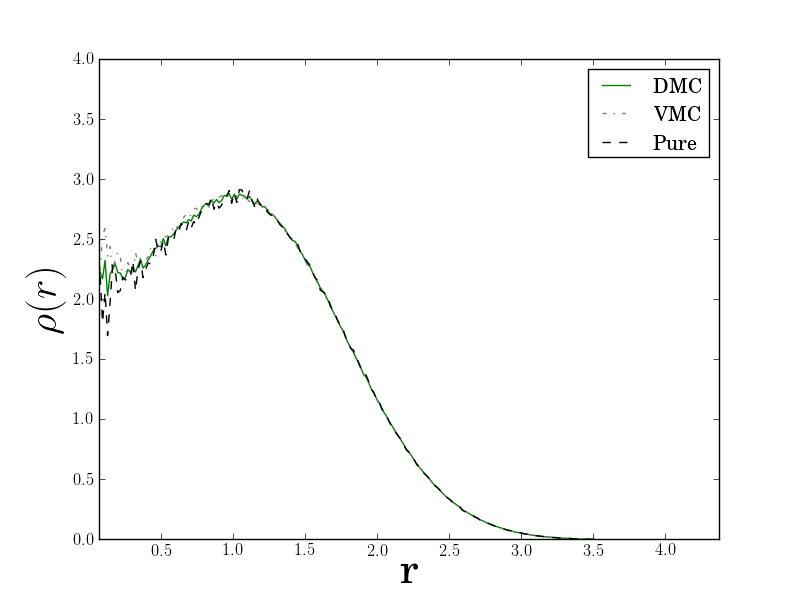
\includegraphics[scale=0.17]{../graphics/OBD/OBD_Q3D/QD8w1_2D.png}} \\
   \footnotesize{\rot{$\quad\,\,\omega=0.01$}}&\subfigure{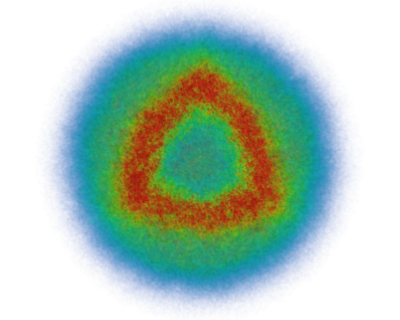
\includegraphics[scale=0.2]{../graphics/OBD/OBD_Q3D/QD8w001_3D.png}} 
   \subfigure{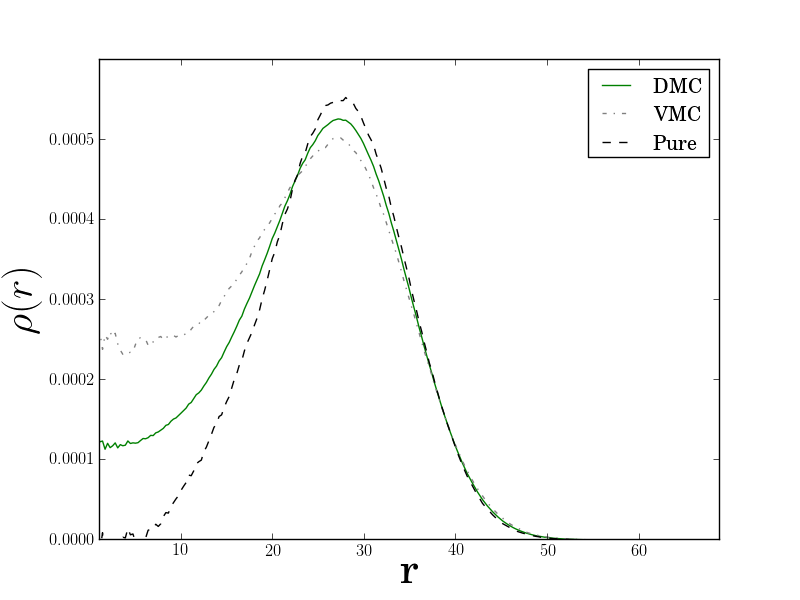
\includegraphics[scale=0.17]{../graphics/OBD/OBD_Q3D/QD8w001_2D.png}} 
  \end{tabular}
  \caption{One-body densities for a 8-particle three-dimensional quantum dot for high and low frequencies.}
  \label{fig:OBD_QDOTS3D_lowfreq}
 \end{center}
\end{figure}
\def\arraystretch{1}
\end{frame}


\begin{frame}

\captionsetup[subfloat]{labelformat=empty}

\tiny
\begin{figure}
 \begin{center}
 \begin{tabular}{rl}
  \rot{$\qquad\omega=0.28$}&\subfigure{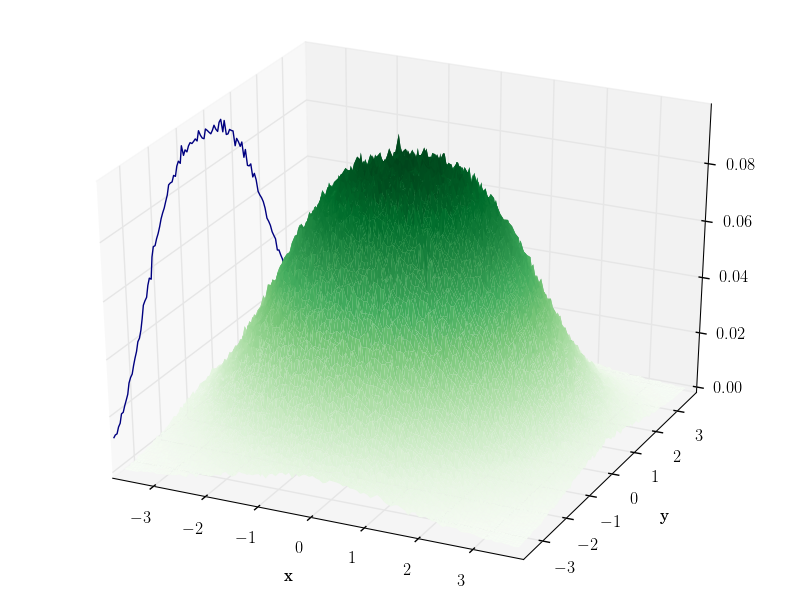
\includegraphics[scale=\OBDscale]{../graphics/OBD/OBD_DMC/dist_out_QDots2c028_3D.png}}
  \subfigure{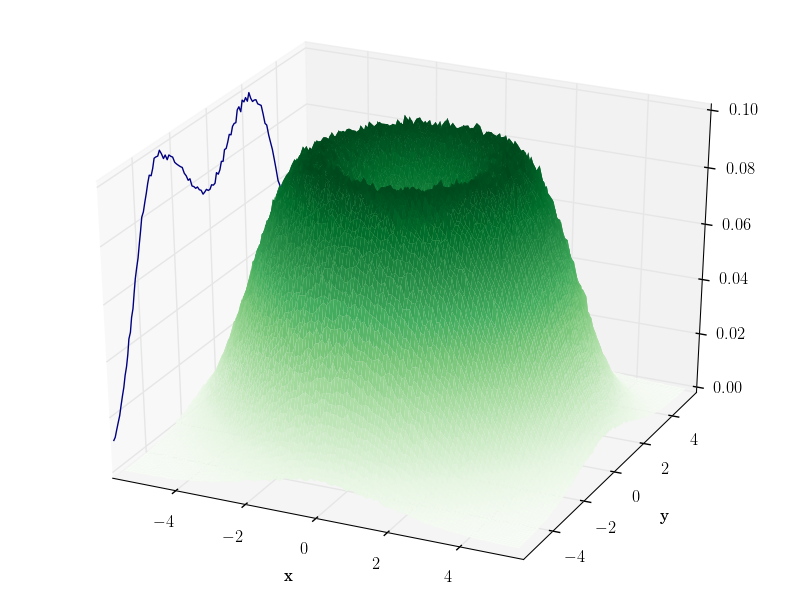
\includegraphics[scale=\OBDscale]{../graphics/OBD/OBD_DMC/dist_out_QDots6c028_3D.png}} 
  \subfigure{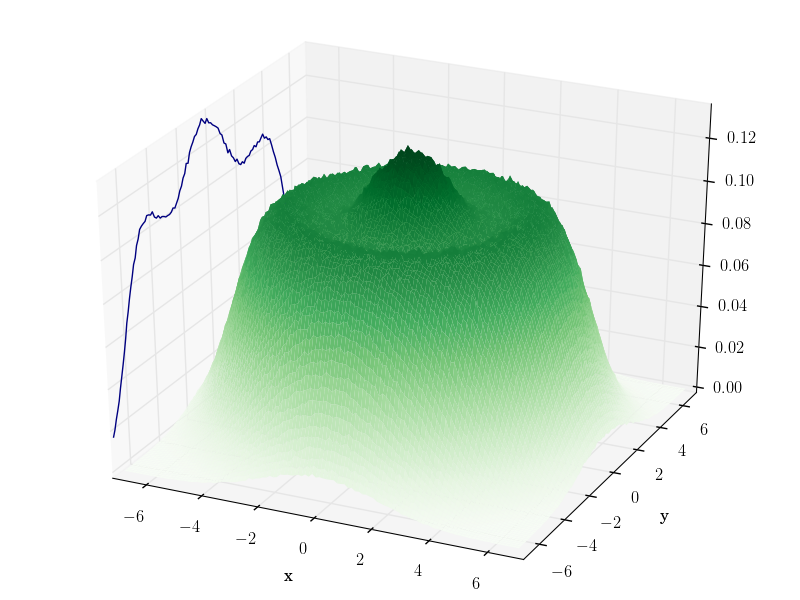
\includegraphics[scale=\OBDscale]{../graphics/OBD/OBD_DMC/dist_out_QDots12c028_3D.png}}
  \subfigure{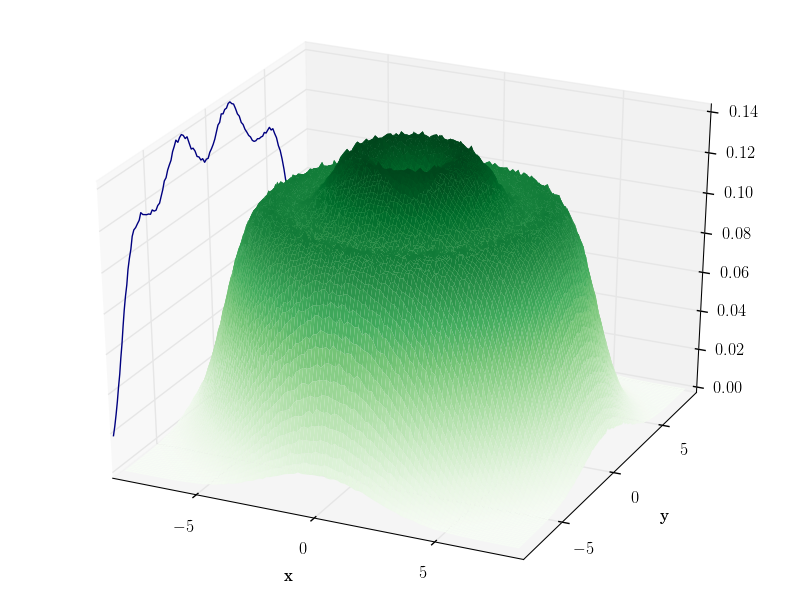
\includegraphics[scale=\OBDscale]{../graphics/OBD/OBD_DMC/dist_out_QDots20c028_3D.png}} \\[-0pt]
  \rot{$\qquad\omega=0.1$}&\subfigure{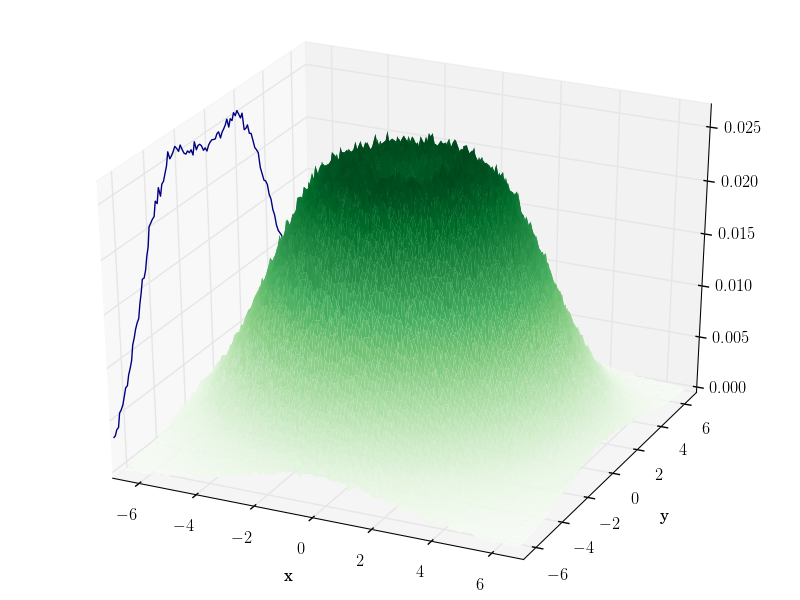
\includegraphics[scale=\OBDscale]{../graphics/OBD/OBD_DMC/dist_out_QDots2c01_3D.png}}
  \subfigure{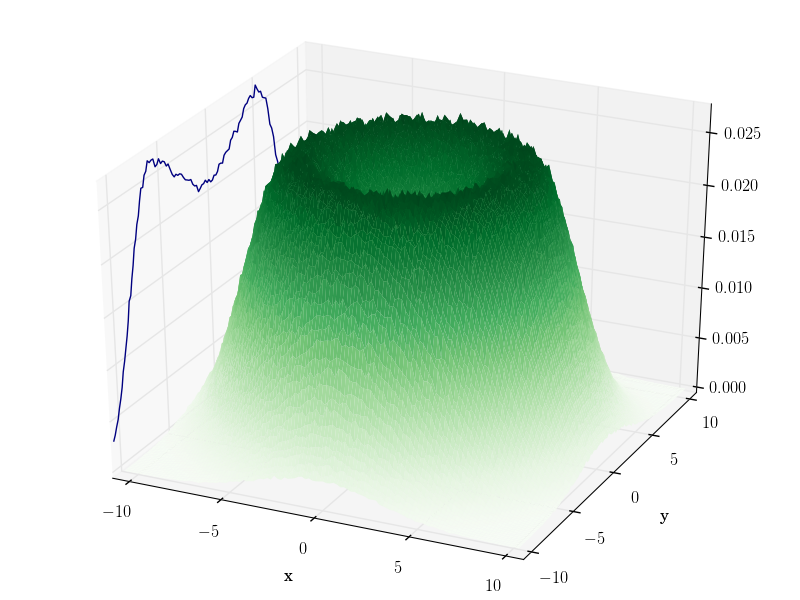
\includegraphics[scale=\OBDscale]{../graphics/OBD/OBD_DMC/dist_out_QDots6c01_3D.png}} 
  \subfigure{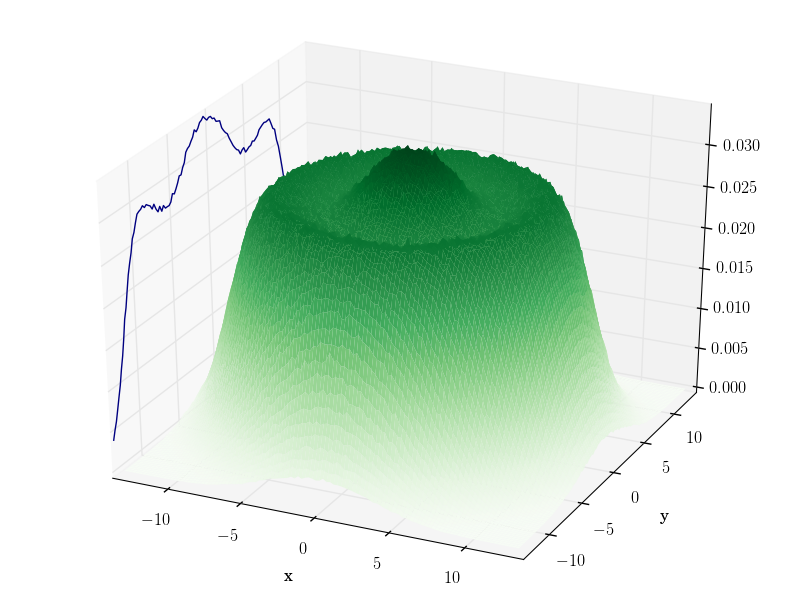
\includegraphics[scale=\OBDscale]{../graphics/OBD/OBD_DMC/dist_out_QDots12c01_3D.png}}
  \subfigure{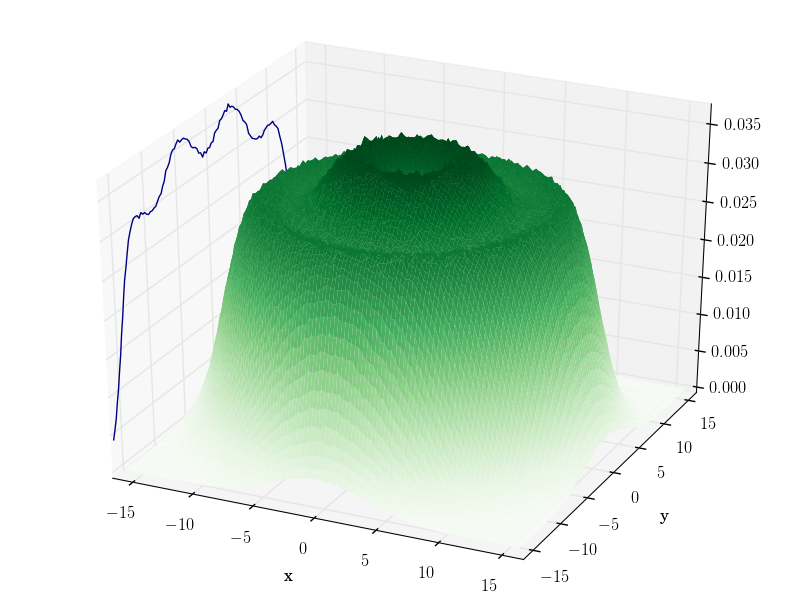
\includegraphics[scale=\OBDscale]{../graphics/OBD/OBD_DMC/dist_out_QDots20c01_3D.png}} \\[-0pt]
  \rot{$\qquad\omega=0.01$}&\subfigure[$N=2$]{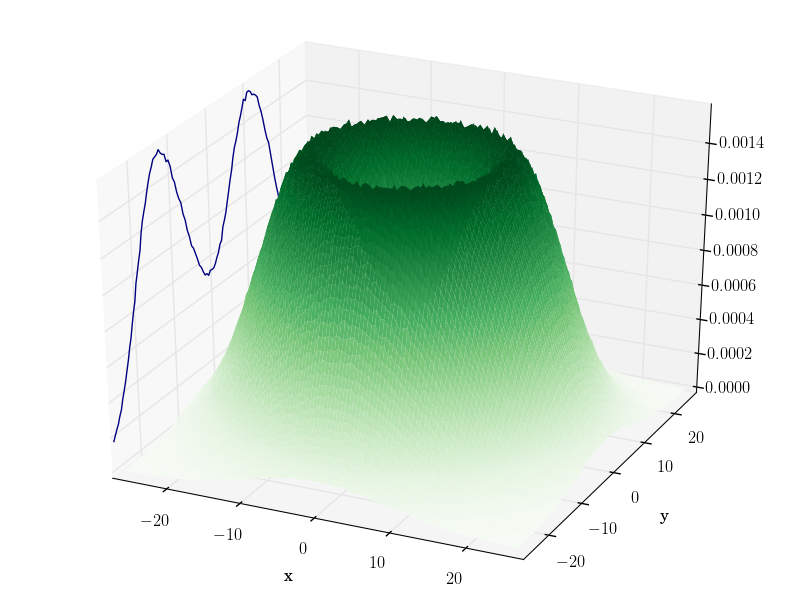
\includegraphics[scale=\OBDscale]{../graphics/OBD/OBD_DMC/dist_out_QDots2c001_3D.png}}
  \subfigure[$N=6$]{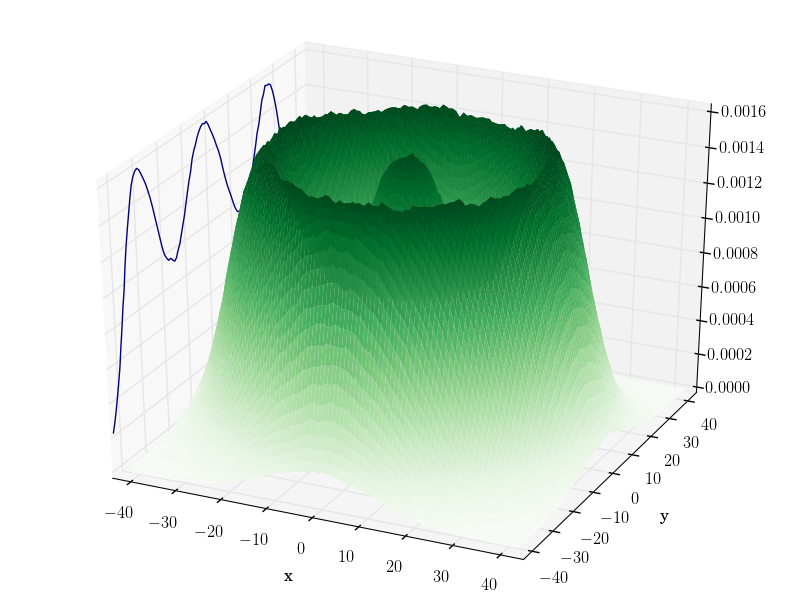
\includegraphics[scale=\OBDscale]{../graphics/OBD/OBD_DMC/dist_out_QDots6c001_3D.png}} 
  \subfigure[$N=12$]{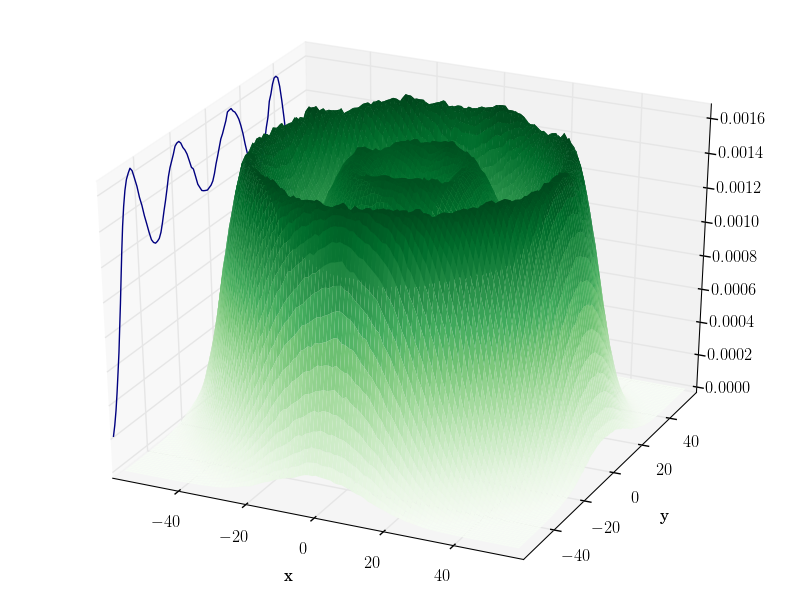
\includegraphics[scale=\OBDscale]{../graphics/OBD/OBD_DMC/dist_out_QDots12c001_3D.png}}
  \subfigure[$N=20$]{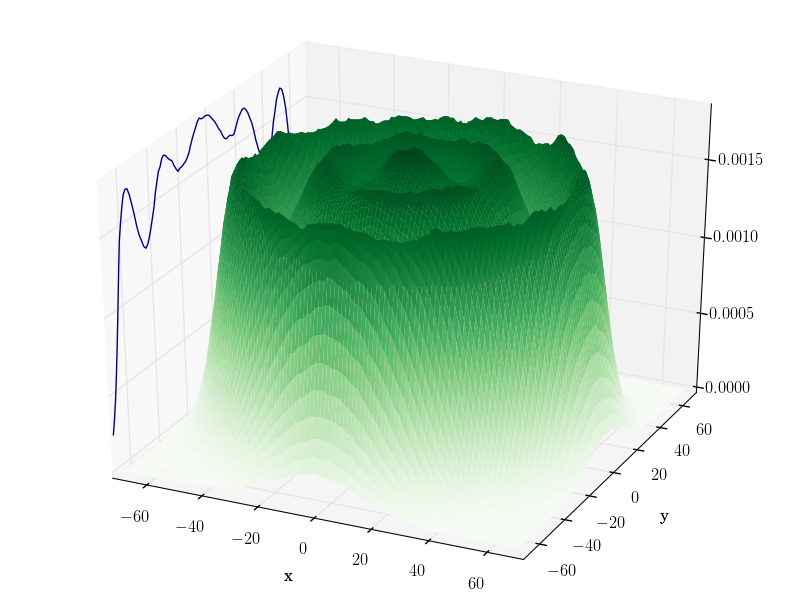
\includegraphics[scale=\OBDscale]{../graphics/OBD/OBD_DMC/dist_out_QDots20c001_3D.png}} \\
 \end{tabular}
  \label{fig:OBD_DMC_QDOTS_lowering3D}
 \end{center}
\end{figure}
\setlength{\tabcolsep}{6pt}
\normalsize

\end{frame}

\begin{frame}
 The electrons become more \textit{localized} and dilute. 
 \shift
 
 The two- and three-dimensional densities no longer match.
 \shift
 
 Transition into a new region? 
\end{frame}


\begin{frame}
\frametitle{Electron crystals for N=6}
 \begin{figure}
 \begin{center}
  \subfigure{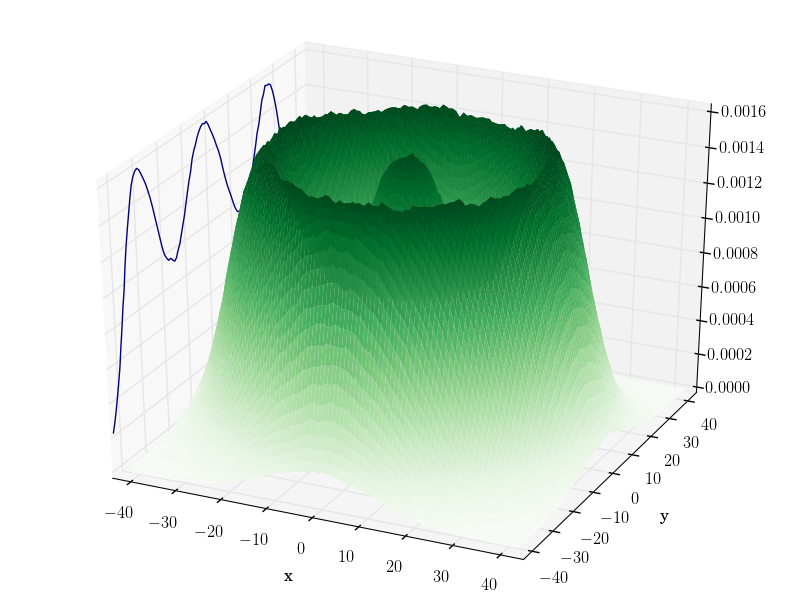
\includegraphics[scale=0.25]{../graphics/OBD/OBD_DMC/dist_out_QDots6c001_3D.png}}
  \subfigure{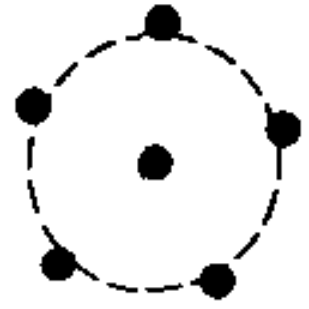
\includegraphics[scale=0.2]{../graphics/wigner/wigner6.png}}
  \label{fig:wigner20}
  \caption{OBD for a 6-particle two-dimensional quantum dot compared to the classical theoretical configuration taken from F. Bolton, U. Rössler.  \textit{Superlattices and microstructures} \textbf{13}, 139 (1993).}
 \end{center}
\end{figure}
\end{frame}

\begin{frame}
\frametitle{Electron crystals for N=6 (frozen)}
 \begin{figure}
 \begin{center}
  \subfigure{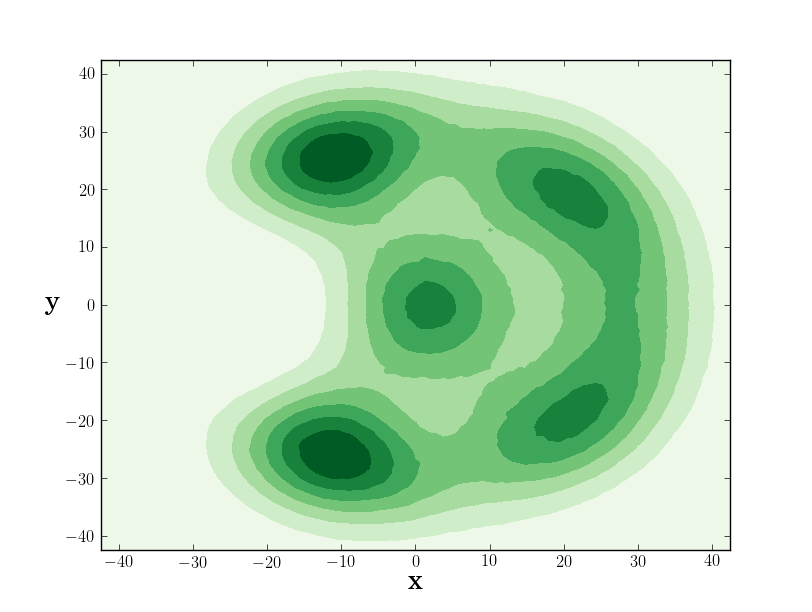
\includegraphics[scale=0.25]{../graphics/wigner/locked6_2d.png}}
  \subfigure{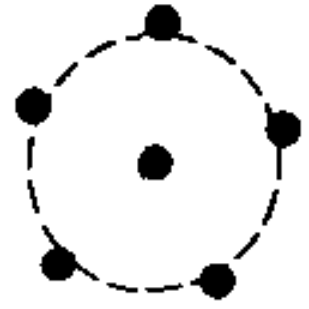
\includegraphics[scale=0.2]{../graphics/wigner/wigner6.png}}
  \label{fig:wigner20}
  \caption{OBD for a 6-particle two-dimensional quantum dot compared to the classical theoretical configuration taken from F. Bolton, U. Rössler.  \textit{Superlattices and microstructures} \textbf{13}, 139 (1993).}
 \end{center}
\end{figure}
\end{frame}

\begin{frame}
\frametitle{Electron crystals for N=6 (frozen)}
 \begin{figure}
 \begin{center}
  \subfigure{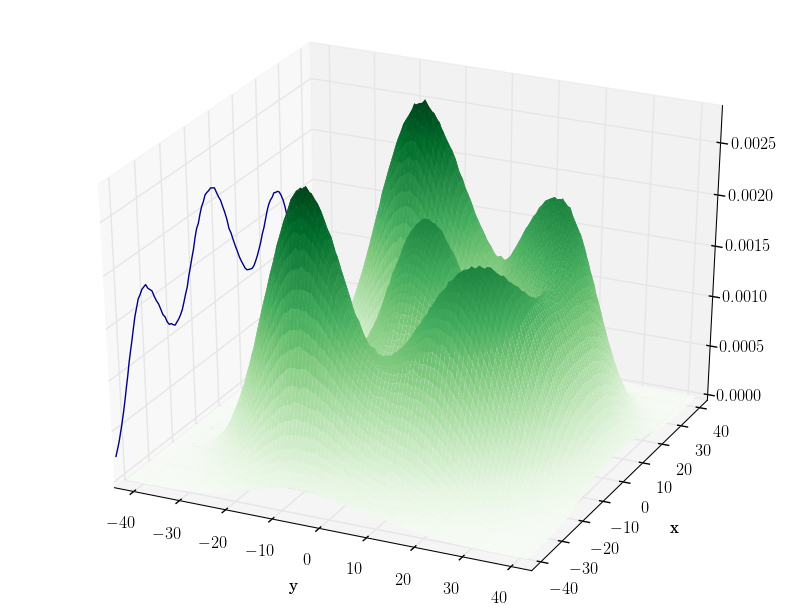
\includegraphics[scale=0.25]{../graphics/wigner/locked6_3d.png}}
  \subfigure{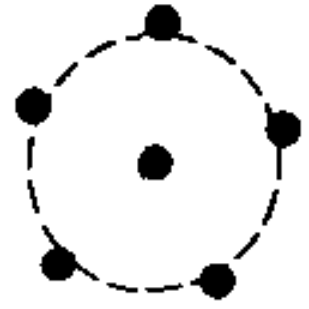
\includegraphics[scale=0.2]{../graphics/wigner/wigner6.png}}
  \label{fig:wigner20}
  \caption{OBD for a 6-particle two-dimensional quantum dot compared to the classical theoretical configuration taken from F. Bolton, U. Rössler.  \textit{Superlattices and microstructures} \textbf{13}, 139 (1993).}
 \end{center}
\end{figure}
\end{frame}

\begin{frame}
\frametitle{Electron crystals for N=12}
 \begin{figure}
 \begin{center}
  \subfigure{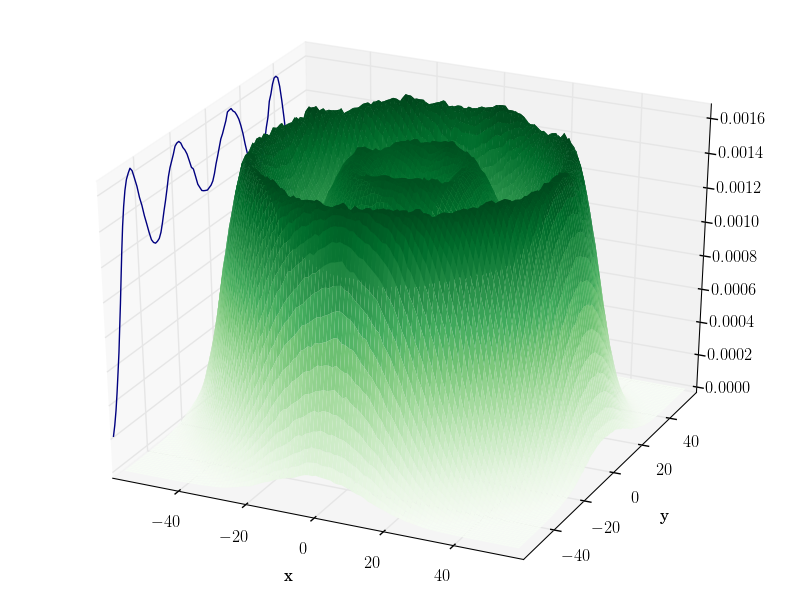
\includegraphics[scale=0.25]{../graphics/OBD/OBD_DMC/dist_out_QDots12c001_3D.png}}
  \subfigure{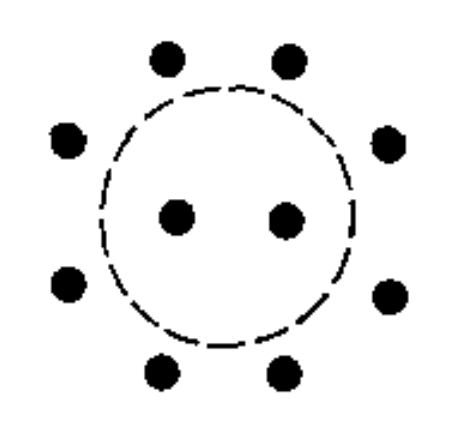
\includegraphics[scale=0.2]{../graphics/wigner/wigner10.png}}
  \label{fig:wigner20}
  \caption{OBD for a 12-particle two-dimensional quantum dot compared to the classical theoretical configuration taken from F. Bolton, U. Rössler.  \textit{Superlattices and microstructures} \textbf{13}, 139 (1993).}
 \end{center}
\end{figure}
\end{frame}

\begin{frame}
\frametitle{Electron crystals for N=12 (frozen)}
 \begin{figure}
 \begin{center}
  \subfigure{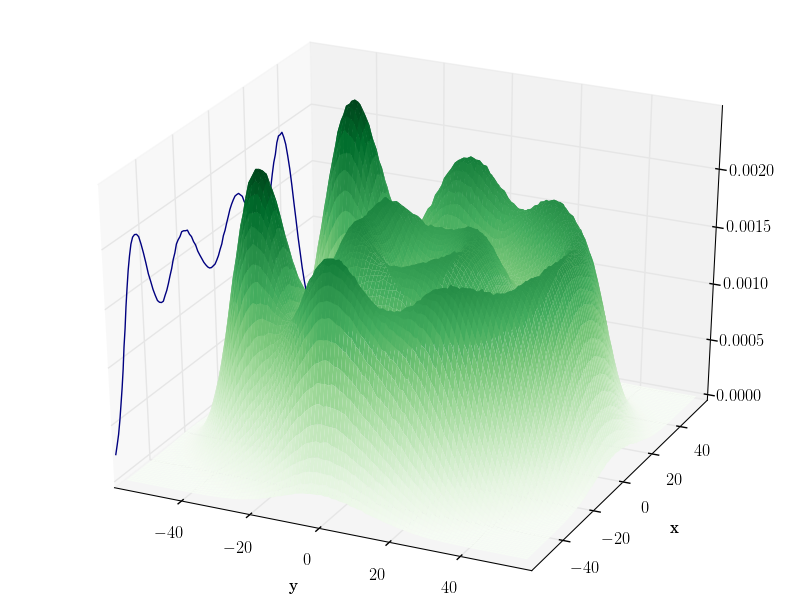
\includegraphics[scale=0.25]{../graphics/wigner/locked12_3d.png}}
  \subfigure{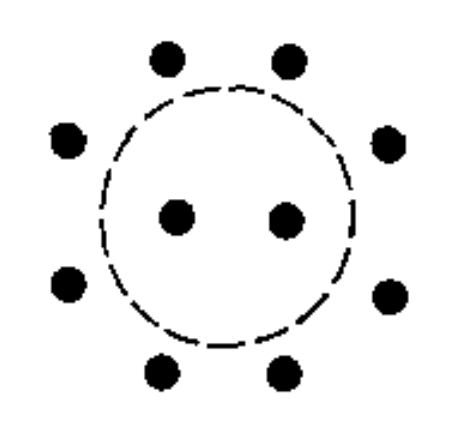
\includegraphics[scale=0.2]{../graphics/wigner/wigner10.png}}
  \label{fig:wigner20}
  \caption{OBD for a 12-particle two-dimensional quantum dot compared to the classical theoretical configuration taken from F. Bolton, U. Rössler.  \textit{Superlattices and microstructures} \textbf{13}, 139 (1993).}
 \end{center}
\end{figure}
\end{frame}


\begin{frame}
\frametitle{Electron crystals N=20}
 \begin{figure}
 \begin{center}
  \subfigure{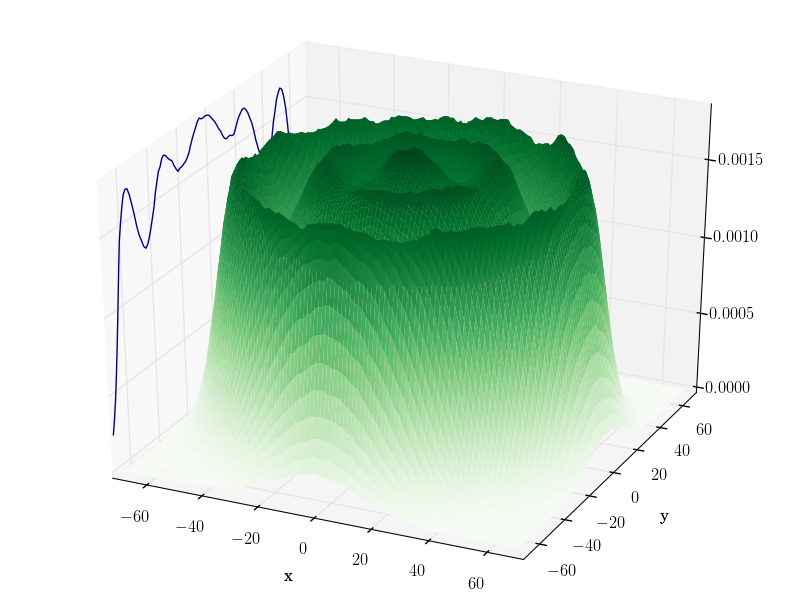
\includegraphics[scale=0.25]{../graphics/OBD/OBD_DMC/dist_out_QDots20c001_3D.png}}
  \subfigure{\includegraphics[scale=0.15]{../graphics/wigner/wigner20.png}}
  \label{fig:wigner20}
  \caption{OBD for a 20-particle two-dimensional quantum dot compared to the classical theoretical configuration taken from P. Galatola et al.~\textit{Eur. Phys. J. B} \textbf{50}, 549 (2006).}
 \end{center}
\end{figure}
\end{frame}

\begin{frame}
 This effect is called \textit{Wigner Crystallization} and is expected for low density electron gases when the \textbf{kinetic energy on average becomes far lower than the corresponding total potential energy}.
 \shift
 
 The connection between potential and kinetic energy is given by the \textit{virial theorem}
 
 \begin{equation}
  V(\mathbf{r}) \propto r^\gamma \quad\longrightarrow\quad \langle \OP{T} \rangle = \frac{\gamma}{2} \langle \OP{V} \rangle, \label{eq:virial}
 \end{equation}
 \shift
 
 Systems with similar proportionality constant follow the same effective potential, that is, they have similar eigenstates.

\end{frame}

\begin{frame}
 \captionsetup[subfloat]{labelformat=empty}
\begin{figure}[h]
 \begin{center}
  \subfigure[$N=6$]{\includegraphics[scale=0.25]{../graphics/VirialPlots/E_vs_w_E6.png}}
  \subfigure[$N=42$]{\includegraphics[scale=0.25]{../graphics/VirialPlots/E_vs_w_E42.png}} \\
  \caption{The relative magnitude of the expectation value of the different energy sources as a function of the frequency $\omega$ (left) together with the magnitude of the sources' energy contributions scaled with the oscillator frequency (right).}
  \label{fig:E_dist_qdots}
 \end{center}
\end{figure}
\end{frame}

% 
% \begin{frame}
%  Conclusions:
%  \shift
%  The kinetic energy falls whereas the total potential energy increases.
%  \shift
%  The kinetic energy is proportional to the frequency
%  
%  \begin{equation}
%   \langle \OP{T} \rangle \propto \omega.
%  \end{equation}
%  
% \end{frame}

\begin{frame}
 \frametitle{Transition into a Wigner crystal?} 
 \captionsetup[subfloat]{labelformat=empty}
 \begin{figure}[h]
 \begin{center}
  \subfigure[$N=6$]{\includegraphics[scale=0.3]{../graphics/VirialPlots/E_vs_w_V6.png}}
  \subfigure[$N=42$]{\includegraphics[scale=0.3]{../graphics/VirialPlots/E_vs_w_V42.png}} \\
  \caption{The total kinetic energy vs. the total potential energy of two dimensional quantum dots. NB: Collapsed.}
  \label{fig:V_dist_qdots}
 \end{center}
\end{figure}
\captionsetup[subfloat]{labelformat=parens}
\end{frame}

\begin{frame}
 \frametitle{Preliminary double-well density}
 
 \begin{figure}[h]
 \begin{center}
 \includegraphics[scale=0.25]{../graphics/DoubleWell.png}
  \caption{A countour plot of the trial wave function for a two-particle double-well quantum dot with the wells separated at a distance $R = 2$.}
  \label{fig:doubleWell}
 \end{center}
\end{figure}
 
\end{frame}


\subsection{Atomic systems}

\footnotesize
\begin{frame}
\frametitle{Atoms}
 \begin{table}
\begin{center}
\begin{tabular}{lp{1cm}ccl}
Atom (N) & & $E_\mathrm{VMC}$ & \qquad $E_\mathrm{DMC}$ & \qquad\,\, Expt. \\
\hline\hline
\ \\
He (2) & \qquad & -2.8903(2) & \qquad -2.9036(2) & \qquad $-2.9037$ \\
\ \\
% Be & \qquad & -14.145(2) & \qquad -14.657(2)  & \qquad $-14.6674$\\
% \ \\
% Ne & \qquad & -127.853(2) & \qquad -128.765(4) & \qquad $-128.9383$  \\
% \ \\
% Mg & \qquad & -197.269(3) & \qquad -199.904(8) & \qquad $-200.054$  \\
% \ \\
% Ar & \qquad & -524.16(7) & \qquad -527.30(4) & \qquad $-527.544$   \\
% \ \\
Kr (36) & \qquad & -2700(5) & \qquad -2749.9(2) & \qquad $-2752.054976$  \\
\ \\
\end{tabular}
\caption{Ground state energies for atoms calculated using Variational - and Diffusion Monte-Carlo.}
\label{tab:AtomsRes}
\end{center}
\end{table}
\normalsize
\end{frame}

% \begin{frame}
%  Quantum dots results for VMC and DMC were significantly more similar. 
%  \shift
%  Worse for the non-noble gases and for higher number of particles.
%  \shift
%  Easier to excite an electron into the next sub-shell (next $l$) than to the next $n$.
%  \shift
%  The hydrogenic ansatz only accounts for \textit{bound states}. 
% \end{frame}

\begin{frame}
\frametitle{Densities: The noble gases}
 \begin{figure}
 \begin{center}
   \subfigure{\includegraphics[scale=0.3]{../graphics/OBD/OBD_Atoms/3D/Helium.png}} 
%    \subfigure{\includegraphics[scale=0.15]{../graphics/OBD/OBD_Atoms/2D/Helium.png}}  \\
   \subfigure{\includegraphics[scale=0.3]{../graphics/OBD/OBD_Atoms/3D/Neon.png}} 
%    \subfigure{\includegraphics[scale=0.15]{../graphics/OBD/OBD_Atoms/2D/Neon.png}}  \\
%    \subfigure{\includegraphics[scale=0.4]{../graphics/OBD/OBD_Atoms/3D/Argon.png}} 
%    \subfigure{\includegraphics[scale=0.3]{../graphics/OBD/OBD_Atoms/2D/Argon.png}}  \\
%    \subfigure{\includegraphics[scale=0.2]{../graphics/OBD/OBD_Atoms/3D/Krypton.png}} 
%    \subfigure{\includegraphics[scale=0.15]{../graphics/OBD/OBD_Atoms/2D/Krypton.png}}  \\
  \caption{One-body densities for helium and neon. }
  \label{fig:OBD_noble_Atoms_2D_combo}
 \end{center}
\end{figure}
\end{frame}



\begin{frame}
\frametitle{Densities: The alkaline earth metals}
  \begin{figure}
 \begin{center}
   \subfigure{\includegraphics[scale=0.3]{../graphics/OBD/OBD_Atoms/3D/Beryllium.png}} 
%    \subfigure{\includegraphics[scale=0.15]{../graphics/OBD/OBD_Atoms/2D/Beryllium.png}}  \\
   \subfigure{\includegraphics[scale=0.3]{../graphics/OBD/OBD_Atoms/3D/Magnesium.png}} 
%    \subfigure{\includegraphics[scale=0.15]{../graphics/OBD/OBD_Atoms/2D/Magnesium.png}}  \\
  \caption{Three dimensional one-body density for alkaline earth metals; beryllium  and magnesium.}
  \label{fig:OBD_alkaline_Atoms_2D_combo}
 \end{center}
\end{figure}
\end{frame}

\begin{frame}
\frametitle{Molecules}
 \begin{table}
\begin{center}
\begin{tabular}{lcccrlrr}
Molecule (N) & $R$ & & \qquad & $E_\mathrm{VMC}$ & & \qquad $E_\mathrm{DMC}$ & \qquad\,\, Expt.\\
\hline\hline
\ \\
$\mathrm{H_2}$ (2) & 1.4   & &\qquad & -1.1551(3)    & \qquad   & -1.1745(3)   & \qquad $-1.1746$     \\
\ \\
% $\mathrm{Li_2}$& 5.051 & &\qquad & -14.743(3)    & \qquad   & -14.988(2)   & \qquad $-14.99544$     \\
% \ \\
% $\mathrm{Be_2}$& 4.63  & &\qquad & -28.666(5)    & \qquad   & -29.301(5)   & \qquad $-29.33854(5)$  \\
% \ \\
% $\mathrm{B_2}$ & 3.005 & &\qquad & -47.746(7)    & \qquad   & -49.155(5)   & \qquad $-49.4184$    \\
% \ \\
% $\mathrm{C_2}$ & 2.3481& &\qquad & -72.590(8)    & \qquad   & -74.95(1)    & \qquad $-75.923(5)$   \\
% \ \\
% $\mathrm{N_2}$ & 2.068 & &\qquad & -102.78(1)    & \qquad   & -106.05(2)   & \qquad $-109.5423$    \\
% \ \\
$\mathrm{O_2}$ (16) & 2.282 & &\qquad & -143.97(2)    & \qquad   & -148.53(2)   & \qquad $-150.3268$    \\
\ \\
\end{tabular}
\caption{Ground state energies for homonuclear diatomic molecules calculated using VMC and DMC. }
\label{tab:MoleculesRes}
\end{center}
\end{table}
\end{frame}


\begin{frame}
 \begin{figure}[h]
 \begin{center}
   \subfigure{\includegraphics[scale=0.2]{../graphics/OBD/OBD_MOL/Li2_3D.png}} 
   \subfigure{\includegraphics[scale=0.15]{../graphics/OBD/OBD_MOL/Li2_2D.png}}  \\
   \subfigure{\includegraphics[scale=0.2]{../graphics/OBD/OBD_MOL/O2_3D.png}} 
   \subfigure{\includegraphics[scale=0.15]{../graphics/OBD/OBD_MOL/O2_2D.png}}
  \caption{One-body densities of $\mathrm{Li_2}$ (top) and $\mathrm{O_2}$ (bottom). }
  \label{fig:OBD_Molecules}
 \end{center}
\end{figure}
\end{frame}

% \begin{frame}
%  \frametitle{Parameterizing Force-field Potentials}
% 
% The potential energy in a molecular dynamics simulation is \emph{any energy source which can be used to alter the kinetic energy of the atoms}.
% \shift
% 
% The electrons are not simulated, hence the \emph{total energy of the quantum mechanical system correspond to the molecular potential}.
% 
% \begin{equation}
%  F_\mathrm{MD}(R) = \frac{\mathrm{d} V_\mathrm{MD}}{\mathrm{d} R} = \frac{\mathrm{d} E}{\mathrm{d} R}.
% \end{equation}
% \shift
% 
% This energy vs. $R$ relation can be parameterized using Quantum Monte-Carlo.
% 
% 
% \end{frame}

\begin{frame}
\frametitle{Parameterizing force-field potentials}
 \begin{figure}
 \begin{center}
  \includegraphics[scale=0.5]{../graphics/R_VS_E/LD.png}
  \caption{The Lennard-Jones 12-6 potential.}
  \label{fig:LennardJones}
   \end{center}
\end{figure}
\end{frame}

\begin{frame}
\frametitle{Parameterizing force-field potentials}
 \captionsetup[subfloat]{labelformat=empty}
 \begin{figure}
 \begin{center}
  \subfigure[$\mathrm{H_2}$]{\includegraphics[scale=0.25]{../graphics/R_VS_E/R_vs_E_hyd_pure.png}}
  \subfigure[$\mathrm{Li_2}$]{\includegraphics[scale=0.25]{../graphics/R_VS_E/R_vs_E_lit_pure.png}} 
  \caption{The distance between the atoms $R$ vs. the potential and total energy calculated using QMC.}
  \label{fig:molecules_R_vs_E}
 \end{center}
\end{figure}
\end{frame}



 















\begin{frame}
 \frametitle{Prospects and future work}
 \begin{itemize}
  \item Investigate the similarities between two- and three-dimensional quantum dots in greater detail.
  \item Perform a detailed QMC analysis of double-well quantum dots.
  \item Study more complicated molecules.
  \begin{itemize}
  \item Expand the code to general molecules.
  \item Obtain a better atomic trial wave function by using \textit{Hartree-Fock} or Coupled Cluster wave functions.
  \end{itemize}
  \item Implement a momentum space version of QMC for studying nuclear interactions in great detail.
 \end{itemize}

\end{frame}
\end{document}
